\documentclass[12pt]{article}

\usepackage{sbc-template}
\usepackage[brazil]{babel}
\usepackage[utf8]{inputenc}
\usepackage[T1]{fontenc}
\usepackage{graphicx,url,amsmath,amssymb,booktabs,multirow}
\usepackage[hidelinks]{hyperref}
\usepackage{enumitem}
\setlist{itemsep=1pt,topsep=3pt,parsep=0pt}
\graphicspath{{../figuras/}}

\newcommand{\nomeautor}{Cledson da Silva Araújo}
% Gerado por relatorio/gerar_numeros.py — não editar à mão.
\newcommand{\nNV}{1.560.938}
\newcommand{\nObitosSIM}{13.471}
\newcommand{\nPareados}{12.155}
\newcommand{\pctPareado}{90,2\%}
\newcommand{\pctPareadoMin}{88,5\%}
\newcommand{\pctPareadoMax}{91,6\%}
\newcommand{\tmnSIM}{8,63}
\newcommand{\tmnPareada}{7,79}
\newcommand{\nPassadas}{6}
\newcommand{\pctParesUmDois}{82\%}
\newcommand{\falsosUmDoisMax}{8\%}
\newcommand{\falsosMax}{31\%}
\newcommand{\falsosPonderado}{6\%}
\newcommand{\anoIni}{2017}
\newcommand{\anoFim}{2024}
\newcommand{\anoObFim}{2025}
\newcommand{\anoValid}{2023}
\newcommand{\anoAjFim}{2022}
\newcommand{\anoTeste}{2024}
\newcommand{\nAjuste}{1.221.071}
\newcommand{\obAjuste}{9.405}
\newcommand{\tmnAjuste}{7,70}
\newcommand{\nValid}{176.145}
\newcommand{\obValid}{1.444}
\newcommand{\tmnValid}{8,20}
\newcommand{\nTeste}{163.722}
\newcommand{\obTeste}{1.306}
\newcommand{\tmnTeste}{7,98}
\newcommand{\razaoEscol}{1,6}
\newcommand{\nVarsA}{28}
\newcommand{\nVarsB}{17}
\newcommand{\ALrAuroc}{0,963}
\newcommand{\ALrAurocIC}{0,963 (0,956--0,969)}
\newcommand{\ALrAuprc}{0,551}
\newcommand{\ALrAuprcIC}{0,551 (0,526--0,579)}
\newcommand{\ALrFum}{0,554}
\newcommand{\ALrFumIC}{0,554 (0,534--0,574)}
\newcommand{\ALrPrec}{0,534}
\newcommand{\ALrPrecIC}{0,534 (0,514--0,556)}
\newcommand{\ALrSens}{0,577}
\newcommand{\ALrSensIC}{0,577 (0,549--0,600)}
\newcommand{\ALrEspec}{0,996}
\newcommand{\ALrEspecIC}{0,996 (0,996--0,996)}
\newcommand{\ALrVpn}{0,997}
\newcommand{\ALrVpnIC}{0,997 (0,996--0,997)}
\newcommand{\ALrBrier}{0,0049}
\newcommand{\ALrBrierIC}{0,0049 (0,0047--0,0051)}
\newcommand{\ALrTop}{88\%}
\newcommand{\ALrOE}{0,93}
\newcommand{\AXgbAuroc}{0,964}
\newcommand{\AXgbAurocIC}{0,964 (0,958--0,970)}
\newcommand{\AXgbAuprc}{0,603}
\newcommand{\AXgbAuprcIC}{0,603 (0,577--0,628)}
\newcommand{\AXgbFum}{0,604}
\newcommand{\AXgbFumIC}{0,604 (0,583--0,625)}
\newcommand{\AXgbPrec}{0,597}
\newcommand{\AXgbPrecIC}{0,597 (0,576--0,620)}
\newcommand{\AXgbSens}{0,610}
\newcommand{\AXgbSensIC}{0,610 (0,583--0,636)}
\newcommand{\AXgbEspec}{0,997}
\newcommand{\AXgbEspecIC}{0,997 (0,996--0,997)}
\newcommand{\AXgbVpn}{0,997}
\newcommand{\AXgbVpnIC}{0,997 (0,997--0,997)}
\newcommand{\AXgbBrier}{0,0045}
\newcommand{\AXgbBrierIC}{0,0045 (0,0043--0,0047)}
\newcommand{\AXgbTop}{88\%}
\newcommand{\AXgbOE}{0,95}
\newcommand{\ALgbmAuroc}{0,964}
\newcommand{\ALgbmAurocIC}{0,964 (0,958--0,970)}
\newcommand{\ALgbmAuprc}{0,580}
\newcommand{\ALgbmAuprcIC}{0,580 (0,552--0,608)}
\newcommand{\ALgbmFum}{0,596}
\newcommand{\ALgbmFumIC}{0,596 (0,573--0,617)}
\newcommand{\ALgbmPrec}{0,610}
\newcommand{\ALgbmPrecIC}{0,610 (0,586--0,633)}
\newcommand{\ALgbmSens}{0,583}
\newcommand{\ALgbmSensIC}{0,583 (0,556--0,608)}
\newcommand{\ALgbmEspec}{0,997}
\newcommand{\ALgbmEspecIC}{0,997 (0,997--0,997)}
\newcommand{\ALgbmVpn}{0,997}
\newcommand{\ALgbmVpnIC}{0,997 (0,996--0,997)}
\newcommand{\ALgbmBrier}{0,0046}
\newcommand{\ALgbmBrierIC}{0,0046 (0,0044--0,0048)}
\newcommand{\ALgbmTop}{88\%}
\newcommand{\ALgbmOE}{0,94}
\newcommand{\BLrAuroc}{0,886}
\newcommand{\BLrAurocIC}{0,886 (0,874--0,896)}
\newcommand{\BLrAuprc}{0,366}
\newcommand{\BLrAuprcIC}{0,366 (0,338--0,394)}
\newcommand{\BLrFum}{0,450}
\newcommand{\BLrFumIC}{0,450 (0,429--0,471)}
\newcommand{\BLrPrec}{0,434}
\newcommand{\BLrPrecIC}{0,434 (0,411--0,455)}
\newcommand{\BLrSens}{0,467}
\newcommand{\BLrSensIC}{0,467 (0,442--0,492)}
\newcommand{\BLrEspec}{0,995}
\newcommand{\BLrEspecIC}{0,995 (0,995--0,995)}
\newcommand{\BLrVpn}{0,996}
\newcommand{\BLrVpnIC}{0,996 (0,996--0,996)}
\newcommand{\BLrBrier}{0,0059}
\newcommand{\BLrBrierIC}{0,0059 (0,0058--0,0061)}
\newcommand{\BLrTop}{71\%}
\newcommand{\BLrOE}{0,95}
\newcommand{\BXgbAuroc}{0,891}
\newcommand{\BXgbAurocIC}{0,891 (0,879--0,902)}
\newcommand{\BXgbAuprc}{0,390}
\newcommand{\BXgbAuprcIC}{0,390 (0,360--0,418)}
\newcommand{\BXgbFum}{0,454}
\newcommand{\BXgbFumIC}{0,454 (0,432--0,476)}
\newcommand{\BXgbPrec}{0,470}
\newcommand{\BXgbPrecIC}{0,470 (0,446--0,494)}
\newcommand{\BXgbSens}{0,440}
\newcommand{\BXgbSensIC}{0,440 (0,413--0,464)}
\newcommand{\BXgbEspec}{0,996}
\newcommand{\BXgbEspecIC}{0,996 (0,996--0,996)}
\newcommand{\BXgbVpn}{0,995}
\newcommand{\BXgbVpnIC}{0,995 (0,995--0,996)}
\newcommand{\BXgbBrier}{0,0059}
\newcommand{\BXgbBrierIC}{0,0059 (0,0057--0,0061)}
\newcommand{\BXgbTop}{71\%}
\newcommand{\BXgbOE}{0,96}
\newcommand{\BLgbmAuroc}{0,890}
\newcommand{\BLgbmAurocIC}{0,890 (0,879--0,901)}
\newcommand{\BLgbmAuprc}{0,396}
\newcommand{\BLgbmAuprcIC}{0,396 (0,367--0,424)}
\newcommand{\BLgbmFum}{0,457}
\newcommand{\BLgbmFumIC}{0,457 (0,435--0,481)}
\newcommand{\BLgbmPrec}{0,466}
\newcommand{\BLgbmPrecIC}{0,466 (0,441--0,490)}
\newcommand{\BLgbmSens}{0,448}
\newcommand{\BLgbmSensIC}{0,448 (0,423--0,474)}
\newcommand{\BLgbmEspec}{0,996}
\newcommand{\BLgbmEspecIC}{0,996 (0,996--0,996)}
\newcommand{\BLgbmVpn}{0,996}
\newcommand{\BLgbmVpnIC}{0,996 (0,995--0,996)}
\newcommand{\BLgbmBrier}{0,0059}
\newcommand{\BLgbmBrierIC}{0,0059 (0,0057--0,0060)}
\newcommand{\BLgbmTop}{71\%}
\newcommand{\BLgbmOE}{0,97}
\newcommand{\dAB}{0,074}
\newcommand{\dABIC}{0,064--0,084}
\newcommand{\dXLa}{0,001}
\newcommand{\dXLaIC}{-0,001--0,003}
\newcommand{\dXLb}{0,005}
\newcommand{\dXLbIC}{-0,000--0,011}
\newcommand{\dABprc}{0,214}
\newcommand{\dABprcIC}{0,191--0,241}
\newcommand{\dXLaprc}{0,052}
\newcommand{\dXLaprcIC}{0,040--0,066}
\newcommand{\dXLbprc}{0,024}
\newcommand{\dXLbprcIC}{0,011--0,041}
\newcommand{\oeBrutoA}{0,23}
\newcommand{\arvA}{247}
\newcommand{\profA}{5}
\newcommand{\lrA}{0,036}
\newcommand{\spwA}{11}
\newcommand{\sensAEstAuroc}{0,963}
\newcommand{\sensAEstAuprc}{0,601}
\newcommand{\sensAEstOE}{1,07}
\newcommand{\sensAEstDelta}{-0,0009 (-0,0020 a 0,0001)}
\newcommand{\sensAPiorAuroc}{0,963}
\newcommand{\sensAPiorAuprc}{0,599}
\newcommand{\sensAPiorOE}{1,16}
\newcommand{\sensAPiorDelta}{-0,0013 (-0,0029 a 0,0005)}
\newcommand{\calABruInt}{-2,456 (-2,526 a -2,387)}
\newcommand{\calABruInc}{1,058 (1,029 a 1,088)}
\newcommand{\calACalInt}{-0,082 (-0,154 a -0,011)}
\newcommand{\calACalInc}{1,009 (0,981 a 1,037)}
\newcommand{\nbAUm}{6,6}
\newcommand{\sinalAUm}{5,6\%}
\newcommand{\nbACinco}{5,5}
\newcommand{\sinalACinco}{2,3\%}
\newcommand{\nbAVinte}{4,1}
\newcommand{\sinalAVinte}{1,1\%}
\newcommand{\nbPositivoA}{sim}
\newcommand{\oeBrutoB}{0,17}
\newcommand{\arvB}{407}
\newcommand{\profB}{5}
\newcommand{\lrB}{0,036}
\newcommand{\spwB}{11}
\newcommand{\sensBEstAuroc}{0,891}
\newcommand{\sensBEstAuprc}{0,392}
\newcommand{\sensBEstOE}{1,11}
\newcommand{\sensBEstDelta}{0,0006 (-0,0015 a 0,0029)}
\newcommand{\sensBPiorAuroc}{0,892}
\newcommand{\sensBPiorAuprc}{0,391}
\newcommand{\sensBPiorOE}{1,16}
\newcommand{\sensBPiorDelta}{0,0013 (-0,0009 a 0,0034)}
\newcommand{\calBBruInt}{-2,410 (-2,473 a -2,347)}
\newcommand{\calBBruInc}{1,016 (0,990 a 1,043)}
\newcommand{\calBCalInt}{-0,060 (-0,124 a 0,004)}
\newcommand{\calBCalInc}{0,979 (0,954 a 1,005)}
\newcommand{\nbBUm}{5,3}
\newcommand{\sinalBUm}{7,0\%}
\newcommand{\nbBCinco}{4,0}
\newcommand{\sinalBCinco}{2,4\%}
\newcommand{\nbBVinte}{2,6}
\newcommand{\sinalBVinte}{0,9\%}
\newcommand{\nbPositivoB}{sim}
\newcommand{\driftLog}{0,035}
\newcommand{\posTreinoEstrito}{7.661}
\newcommand{\nNaoPareados}{1.316}
\newcommand{\parPesoAus}{0,8}
\newcommand{\nparPesoAus}{26,8}
\newcommand{\parSemAus}{4,8}
\newcommand{\nparSemAus}{31,5}
\newcommand{\parIdAus}{2,1}
\newcommand{\nparIdAus}{32,2}
\newcommand{\parCap}{35,0}
\newcommand{\nparCap}{19,6}
\newcommand{\parHosp}{98,2}
\newcommand{\nparHosp}{90,2}
\newcommand{\parPesoMed}{1100}
\newcommand{\nparPesoMed}{1400}
\newcommand{\linkCap}{94,3\%}
\newcommand{\linkInt}{88,2\%}
\newcommand{\linkRacaMin}{89,4\%}
\newcommand{\linkRacaMax}{90,6\%}
\newcommand{\linkPesoAus}{20,7\%}
\newcommand{\pctVerdadeiros}{85\%}
\newcommand{\vifFilhos}{20}
\newcommand{\vifGest}{22}
\newcommand{\vifPartos}{4,5}
\newcommand{\vifOutrosMax}{4,6}
\newcommand{\ausCons}{19,7}
\newcommand{\preCons}{7,5}
\newcommand{\pctAusCons}{2,2}
\newcommand{\ausPai}{8,8}
\newcommand{\prePai}{6,6}
\newcommand{\pctAusPai}{54,7}
\newcommand{\ausSem}{13,4}
\newcommand{\preSem}{7,7}
\newcommand{\pctAusSem}{1,1}
\newcommand{\ausApg}{27,6}
\newcommand{\preApg}{7,6}
\newcommand{\pctAusApg}{1,1}
\newcommand{\pctMult}{2,3}
\newcommand{\pctObMult}{10,2}
\newcommand{\aurocUnicosA}{0,963}
\newcommand{\aurocUnicosB}{0,882}
\newcommand{\repo}{https://github.com/CledsonSilvaAraujo/mortalidade-neonatal-rj}
\newcommand{\tempoMin}{41}
\newcommand{\subAAurocMin}{0,950}
\newcommand{\subAAurocMax}{0,980}
\newcommand{\subAFundAuroc}{0,950 (0,932--0,965)}
\newcommand{\subAFundOE}{0,99 (0,90--1,08)}
\newcommand{\subASupAuroc}{0,980 (0,970--0,989)}
\newcommand{\subASupOE}{0,92 (0,84--1,00)}
\newcommand{\subABrancaAuroc}{0,976 (0,966--0,983)}
\newcommand{\subABrancaOE}{0,98 (0,91--1,05)}
\newcommand{\subAPretaAuroc}{0,962 (0,946--0,976)}
\newcommand{\subAPretaOE}{0,92 (0,84--1,01)}
\newcommand{\subACapAuroc}{0,966 (0,954--0,976)}
\newcommand{\subACapOE}{0,91 (0,85--0,97)}
\newcommand{\subAIntAuroc}{0,963 (0,955--0,970)}
\newcommand{\subAIntOE}{0,98 (0,93--1,02)}
\newcommand{\subBAurocMin}{0,875}
\newcommand{\subBAurocMax}{0,906}
\newcommand{\subBFundAuroc}{0,875 (0,846--0,897)}
\newcommand{\subBFundOE}{0,99 (0,90--1,09)}
\newcommand{\subBSupAuroc}{0,902 (0,872--0,928)}
\newcommand{\subBSupOE}{0,94 (0,85--1,05)}
\newcommand{\subBBrancaAuroc}{0,898 (0,877--0,919)}
\newcommand{\subBBrancaOE}{1,02 (0,94--1,11)}
\newcommand{\subBPretaAuroc}{0,906 (0,878--0,929)}
\newcommand{\subBPretaOE}{0,94 (0,85--1,03)}
\newcommand{\subBCapAuroc}{0,885 (0,863--0,906)}
\newcommand{\subBCapOE}{0,94 (0,87--1,02)}
\newcommand{\subBIntAuroc}{0,894 (0,880--0,907)}
\newcommand{\subBIntOE}{0,97 (0,91--1,02)}
\newcommand{\shapTopA}{peso ao nascer, Apgar 5º min, Apgar 1º min, semanas de gestação, anomalia congênita}
\newcommand{\shapTopB}{semanas de gestação, consultas de pré-natal, escolaridade da mãe, apresentação, raça/cor da mãe}
\newcommand{\compTreinoCap}{94,3\%}
\newcommand{\compTesteCap}{94,6\%}
\newcommand{\oeLinkCap}{1,003}
\newcommand{\compDifCap}{0,3}
\newcommand{\oeRegACapBru}{0,22}
\newcommand{\oeRegACapCal}{0,91}
\newcommand{\oeRegBCapBru}{0,17}
\newcommand{\oeRegBCapCal}{0,94}
\newcommand{\compTreinoInt}{88,0\%}
\newcommand{\compTesteInt}{89,6\%}
\newcommand{\oeLinkInt}{1,018}
\newcommand{\compDifInt}{1,6}
\newcommand{\oeRegAIntBru}{0,24}
\newcommand{\oeRegAIntCal}{0,98}
\newcommand{\oeRegBIntBru}{0,17}
\newcommand{\oeRegBIntCal}{0,97}
\newcommand{\testeEstrAAuroc}{0,965}
\newcommand{\testeZeroAAuroc}{0,964}
\newcommand{\nbADois}{6,2}
\newcommand{\nbADez}{4,9}
\newcommand{\testeEstrBAuroc}{0,890}
\newcommand{\testeZeroBAuroc}{0,890}
\newcommand{\nbBDois}{4,7}
\newcommand{\nbBDez}{3,3}
\newcommand{\antABrancaOE}{1,08}
\newcommand{\antAIntOE}{1,05}
\newcommand{\antBBrancaOE}{1,15}
\newcommand{\antBIntOE}{1,08}
\newcommand{\anoTesteAnt}{2023}
\newcommand{\tmnPesoMuitoBaixo}{285}
\newcommand{\tmnPesoNormal}{1,9}
\newcommand{\tmnIgMuitoPrematuro}{262}
\newcommand{\tmnIgTermo}{2,0}
\newcommand{\tmnApgarBaixo}{306}
\newcommand{\xaiSpearA}{0,90}
\newcommand{\xaiTopA}{4}
\newcommand{\xaiMetadesA}{0,999}
\newcommand{\xaiSensA}{3,0\%}
\newcommand{\xaiAditA}{7\times 10^{-6}}
\newcommand{\xaiSpearB}{0,98}
\newcommand{\xaiTopB}{5}
\newcommand{\xaiMetadesB}{0,998}
\newcommand{\xaiSensB}{7,9\%}
\newcommand{\xaiAditB}{6\times 10^{-6}}
\newcommand{\xaiBrancaB}{-0,11}
\newcommand{\xaiPretaB}{0,06}
\newcommand{\xaiEscBaixaB}{0,33}
\newcommand{\xaiEscSupB}{-0,27}
\newcommand{\xaiBase}{6,18\%}
\newcommand{\xaiFnProb}{4,4\%}
\newcommand{\xaiFpProb}{100,0\%}
\newcommand{\xaiVpPeso}{670~g}
\newcommand{\xaiVpApgarUm}{1}
\newcommand{\xaiVpApgarCinco}{1}
\newcommand{\xaiVpSem}{22}
\newcommand{\xaiVpAnom}{com anomalia}
\newcommand{\xaiVpProb}{100,0\%}
\newcommand{\xaiFnPeso}{3.450~g}
\newcommand{\xaiFnApgarUm}{7}
\newcommand{\xaiFnApgarCinco}{8}
\newcommand{\xaiFnSem}{39}
\newcommand{\xaiFnAnom}{com anomalia}
\newcommand{\xaiFpPeso}{385~g}
\newcommand{\xaiFpApgarUm}{1}
\newcommand{\xaiFpApgarCinco}{1}
\newcommand{\xaiFpSem}{21}
\newcommand{\nNVEn}{1,560,938}
\newcommand{\nObitosSIMEn}{13,471}
\newcommand{\pctPareadoEn}{90.2\%}
\newcommand{\pctVerdadeirosEn}{85\%}
\newcommand{\AXgbAurocICEn}{0.964 (95\% CI 0.958--0.970)}
\newcommand{\AXgbAuprcEn}{0.603}
\newcommand{\AXgbTopEn}{88\%}
\newcommand{\BXgbAurocEn}{0.891}
\newcommand{\parUm}{6.043}
\newcommand{\falsosUm}{0\%}
\newcommand{\parDois}{3.917}
\newcommand{\falsosDois}{6--8\%}
\newcommand{\parTres}{846}
\newcommand{\falsosTres}{17--31\%}
\newcommand{\parQuatro}{479}
\newcommand{\falsosQuatro}{12--16\%}
\newcommand{\parCinco}{547}
\newcommand{\falsosCinco}{12--14\%}
\newcommand{\parSeis}{323}
\newcommand{\falsosSeis}{21--22\%}
\newcommand{\prevPareada}{0,78\%}
\newcommand{\hpALr}{0,036}
\newcommand{\hpAMcw}{1,57}
\newcommand{\hpASub}{0,93}
\newcommand{\hpACol}{0,77}
\newcommand{\hpALam}{0,021}
\newcommand{\hpAAlp}{0,002}
\newcommand{\hpAGam}{0,014}
\newcommand{\hpASpw}{11,35}
\newcommand{\hpAProf}{5}
\newcommand{\hpAArv}{247}
\newcommand{\hpBLr}{0,036}
\newcommand{\hpBMcw}{1,57}
\newcommand{\hpBSub}{0,93}
\newcommand{\hpBCol}{0,77}
\newcommand{\hpBLam}{0,021}
\newcommand{\hpBAlp}{0,002}
\newcommand{\hpBGam}{0,014}
\newcommand{\hpBSpw}{11,35}
\newcommand{\hpBProf}{5}
\newcommand{\hpBArv}{407}
\newcommand{\pesoEscolhido}{√(n₀/n₁)}
\newcommand{\tabLinkage}{\begin{tabular}{clrrr}
\toprule
& Chave & Pares & \multicolumn{2}{c}{Falsos pares estimados} \\
\cmidrule(lr){4-5}
& & & Escol. mãe & Perdas fetais \\
\midrule
1 & data + sexo + mun. + peso + id. mãe + sem. gest. + gravidez + parto & 6.043 & 0\% & 0\% \\
2 & data + sexo + mun. + peso + id. mãe & 3.917 & 6\% & 8\% \\
3 & data + sexo + mun. + peso + estab. & 846 & 31\% & 17\% \\
4 & data + sexo + peso + id. mãe & 479 & 12\% & 16\% \\
5 & data + sexo + mun. + id. mãe + sem. gest. & 547 & 14\% & 12\% \\
6 & data + sexo + mun. + estab. + id. mãe & 323 & 21\% & 22\% \\
\bottomrule
\end{tabular}}
\newcommand{\tabMetricas}{\begin{tabular}{llcccccc}
\toprule
Conj. & Modelo & AUROC & AUPRC & F1 & Precisão & Sensib. & Top 5\% \\
\midrule
A & LR & 0,963 (0,956--0,969) & 0,551 (0,526--0,579) & 0,554 & 0,534 & 0,577 & 88\% \\
A & XGBoost & \textbf{0,964 (0,958--0,970)} & \textbf{0,603 (0,577--0,628)} & 0,604 & 0,597 & 0,610 & 88\% \\
A & LightGBM & 0,964 (0,958--0,970) & 0,580 (0,552--0,608) & 0,596 & 0,610 & 0,583 & 88\% \\
\midrule
B & LR & 0,886 (0,874--0,896) & 0,366 (0,338--0,394) & 0,450 & 0,434 & 0,467 & 71\% \\
B & XGBoost & \textbf{0,891 (0,879--0,902)} & \textbf{0,390 (0,360--0,418)} & 0,454 & 0,470 & 0,440 & 71\% \\
B & LightGBM & 0,890 (0,879--0,901) & 0,396 (0,367--0,424) & 0,457 & 0,466 & 0,448 & 71\% \\
\midrule
\multicolumn{2}{l}{Batista et al. (SP)} & 0,971 & 0,586 & 0,548 & 0,729 & 0,440 & $>$90\% \\
\bottomrule
\end{tabular}}
\newcommand{\tabDescritiva}{\begin{tabular}{llrrr}
\toprule
Variável & Categoria & NV & Óbitos & TMN (‰) \\
\midrule
Peso ao nascer & $<$ 1.500 g & 25.466 & 7.268 & 285,4 \\
 & 1.500–2.499 g & 123.814 & 2.136 & 17,3 \\
 & 2.500–3.999 g & 1.335.475 & 2.600 & 1,9 \\
 & $\geq$ 4.000 g & 76.156 & 151 & 2,0 \\
\addlinespace
Idade gestacional & $<$ 32 sem & 26.081 & 6.836 & 262,1 \\
 & 32–36 sem & 150.762 & 2.306 & 15,3 \\
 & 37–41 sem & 1.342.386 & 2.726 & 2,0 \\
 & $\geq$ 42 sem & 23.810 & 48 & 2,0 \\
\addlinespace
Escolaridade da mãe & Fund. incompleto ou menos & 362.104 & 3.404 & 9,4 \\
 & Médio & 834.071 & 6.567 & 7,9 \\
 & Superior & 339.602 & 1.960 & 5,8 \\
\bottomrule
\end{tabular}}
\newcommand{\tabHiper}{\begin{tabular}{lrr}
\toprule
Hiperparâmetro & A · completo & B · pré-parto \\
\midrule
\texttt{learning\_rate} & 0,036 & 0,036 \\
\texttt{max\_depth} & 5 & 5 \\
\texttt{min\_child\_weight} & 1,573 & 1,573 \\
\texttt{subsample} & 0,932 & 0,932 \\
\texttt{colsample\_bytree} & 0,774 & 0,774 \\
\texttt{reg\_lambda} & 0,021 & 0,021 \\
\texttt{reg\_alpha} & 0,002 & 0,002 \\
\texttt{gamma} & 0,014 & 0,014 \\
\texttt{scale\_pos\_weight} & 11,350 & 11,350 \\
\texttt{n\_arvores} & 247 & 407 \\
\bottomrule
\end{tabular}}
\newcommand{\tabVies}{\begin{tabular}{lrr}
\toprule
Característica (na DO) & Pareados & Não pareados \\
\midrule
n & 12.155 & 1.316 \\
Peso ausente (\%) & 0,8 & 26,8 \\
Semanas ausentes (\%) & 4,8 & 31,5 \\
Idade da mãe ausente (\%) & 2,1 & 32,2 \\
Peso mediano (g) & 1.100 & 1.400 \\
Peso $<$ 1.500 g (\%) & 60,2 & 52,1 \\
Óbito no 1º dia (\%) & 26,5 & 31,6 \\
Residente na capital (\%) & 35,0 & 19,6 \\
Óbito em hospital (\%) & 98,2 & 90,2 \\
\bottomrule
\end{tabular}}
\newcommand{\tabSens}{\begin{tabular}{llcccc}
\toprule
Conj. & Rótulos no treino & AUROC & AUPRC & O/E & $\Delta$AUROC (IC 95\%) \\
\midrule
A & principal & 0,964 & 0,603 & 0,95 & -- \\
A & estrito (sem passadas 3--6) & 0,963 & 0,601 & 1,07 & -0,0009 (-0,0020 a 0,0001) \\
A & pior caso (passadas 3--6 = 0) & 0,963 & 0,599 & 1,16 & -0,0013 (-0,0029 a 0,0005) \\
\midrule
B & principal & 0,891 & 0,390 & 0,96 & -- \\
B & estrito (sem passadas 3--6) & 0,891 & 0,392 & 1,11 & 0,0006 (-0,0015 a 0,0029) \\
B & pior caso (passadas 3--6 = 0) & 0,892 & 0,391 & 1,16 & 0,0013 (-0,0009 a 0,0034) \\
\bottomrule
\end{tabular}}
\newcommand{\tabCompletude}{\begin{tabular}{lccccc}
\toprule
Região & Pareamento treino & Pareamento 2024 & O/E esperado & O/E A & O/E B \\
& (2017--2023) & & só pelo linkage & (recalibr.) & (recalibr.) \\
\midrule
Capital & 94,3\% & 94,6\% & 1,003 & 0,91 & 0,94 \\
Interior & 88,0\% & 89,6\% & 1,018 & 0,98 & 0,97 \\
\bottomrule
\end{tabular}}

% Gerado por relatorio_v2/gerar_numeros_v2.py — não editar à mão.
\newcommand{\vBaseTresAuroc}{0,947}
\newcommand{\vBaseTresAuprc}{0,490}
\newcommand{\vBaseTresTop}{84\%}
\newcommand{\vBaseTresDauroc}{0,017 (0,013 a 0,022)}
\newcommand{\vBaseTresDauprc}{0,114 (0,097 a 0,129)}
\newcommand{\vBaseQuatroAuroc}{0,960}
\newcommand{\vBaseQuatroAuprc}{0,522}
\newcommand{\vBaseQuatroTop}{88\%}
\newcommand{\vBaseQuatroDauroc}{0,005 (0,002 a 0,007)}
\newcommand{\vBaseQuatroDauprc}{0,081 (0,064 a 0,097)}
\newcommand{\vIdadeAZero}{0,988}
\newcommand{\vIdadeAZeroTop}{95\%}
\newcommand{\vIdadeAUm}{0,968}
\newcommand{\vIdadeAUmTop}{88\%}
\newcommand{\vIdadeASete}{0,934}
\newcommand{\vIdadeASeteTop}{80\%}
\newcommand{\vIdadeAZeroN}{370}
\newcommand{\vIdadeBZero}{0,921}
\newcommand{\vIdadeBZeroTop}{80\%}
\newcommand{\vIdadeBUm}{0,898}
\newcommand{\vIdadeBUmTop}{70\%}
\newcommand{\vIdadeBSete}{0,848}
\newcommand{\vIdadeBSeteTop}{64\%}
\newcommand{\vIdadeBZeroN}{370}
\newcommand{\vPandAAuroc}{0,964}
\newcommand{\vPandAAuprc}{0,606}
\newcommand{\vPandADauroc}{$-$0,0001 ($-$0,0010 a 0,0007)}
\newcommand{\vPandADauprc}{0,0024 ($-$0,0022 a 0,0075)}
\newcommand{\vChaveAAuroc}{0,956}
\newcommand{\vChaveAAuprc}{0,492}
\newcommand{\vChaveADauroc}{$-$0,0081 ($-$0,0107 a $-$0,0057)}
\newcommand{\vChaveADauprc}{$-$0,1110 ($-$0,1292 a $-$0,0955)}
\newcommand{\vPandBAuroc}{0,889}
\newcommand{\vPandBAuprc}{0,389}
\newcommand{\vPandBDauroc}{$-$0,0014 ($-$0,0045 a 0,0014)}
\newcommand{\vPandBDauprc}{$-$0,0007 ($-$0,0061 a 0,0043)}
\newcommand{\vChaveBAuroc}{0,801}
\newcommand{\vChaveBAuprc}{0,085}
\newcommand{\vChaveBDauroc}{$-$0,0892 ($-$0,0997 a $-$0,0787)}
\newcommand{\vChaveBDauprc}{$-$0,3048 ($-$0,3288 a $-$0,2803)}
\newcommand{\vJanAAurocMin}{0,955}
\newcommand{\vJanAAurocMax}{0,964}
\newcommand{\vJanAOeMin}{0,95}
\newcommand{\vJanAOeMax}{1,01}
\newcommand{\vJanACongOeMin}{0,91}
\newcommand{\vJanACongOeMax}{0,95}
\newcommand{\vJanACongAurocUlt}{0,962}
\newcommand{\vJanAReAurocUlt}{0,964}
\newcommand{\vJanACongIntUlt}{$-$0,16}
\newcommand{\vJanACongOeUlt}{0,91}
\newcommand{\vJanAReOeUlt}{0,95}
\newcommand{\vJanBAurocMin}{0,885}
\newcommand{\vJanBAurocMax}{0,892}
\newcommand{\vJanBOeMin}{0,95}
\newcommand{\vJanBOeMax}{1,05}
\newcommand{\vJanBCongOeMin}{0,93}
\newcommand{\vJanBCongOeMax}{0,99}
\newcommand{\vJanBCongAurocUlt}{0,889}
\newcommand{\vJanBReAurocUlt}{0,891}
\newcommand{\vJanBCongIntUlt}{$-$0,06}
\newcommand{\vJanBCongOeUlt}{0,95}
\newcommand{\vJanBReOeUlt}{0,96}
\newcommand{\vJanAnoIni}{2020}
\newcommand{\vJanAnoFim}{2024}
\newcommand{\vDecPct}{10\%}
\newcommand{\vDecN}{130}
\newcommand{\vDecPctZero}{29\%}
\newcommand{\vDecAZeroDep}{0,990}
\newcommand{\vDecAZeroDepN}{107}
\newcommand{\vDecAZeroAnt}{0,988}
\newcommand{\vDecAZeroAntN}{263}
\newcommand{\vDecAUmDep}{0,986}
\newcommand{\vDecAUmDepN}{23}
\newcommand{\vDecAUmAnt}{0,967}
\newcommand{\vDecAUmAntN}{549}
\newcommand{\vDecBZeroDep}{0,931}
\newcommand{\vDecBZeroDepN}{107}
\newcommand{\vDecBZeroAnt}{0,916}
\newcommand{\vDecBZeroAntN}{263}
\newcommand{\vDecBUmDep}{0,949}
\newcommand{\vDecBUmDepN}{23}
\newcommand{\vDecBUmAnt}{0,896}
\newcommand{\vDecBUmAntN}{549}
\newcommand{\vDigPct}{91\%}
\newcommand{\vFsN}{13}
\newcommand{\vFsCand}{347.020}
\newcommand{\vFsPctTotal}{90,3\%}
\newcommand{\vFsDet}{12.155}
\newcommand{\vFsObitos}{13.471}
\newcommand{\vFsRestantes}{1.316}
\newcommand{\vFsTeste}{0}
\newcommand{\vFsLambda}{0,0036}
\newcommand{\vFsEmLambda}{0,039}
\newcommand{\vFsEmN}{0}
\newcommand{\vFsCompletos}{726}
\newcommand{\vFsPoucos}{269}
\newcommand{\vFsPostBaixo}{901}
\newcommand{\vFsPostBaixoPct}{71\%}
\newcommand{\vFsFalsos}{54\% e 79\%}
\newcommand{\vSimBaixoCob}{98,6\%}
\newcommand{\vSimBaixoFalsos}{0,0\%}
\newcommand{\vSimBaixoSeis}{1\%}
\newcommand{\vSimBaixoSeisEst}{5\%}
\newcommand{\vSimBaixoFsN}{2}
\newcommand{\vSimBaixoFsFalsos}{100\%}
\newcommand{\vSimBaixoMaxTol}{3\%}
\newcommand{\vSimRealCob}{96,7\%}
\newcommand{\vSimRealFalsos}{0,2\%}
\newcommand{\vSimRealSeis}{2\%}
\newcommand{\vSimRealSeisEst}{4\%}
\newcommand{\vSimRealFsN}{15}
\newcommand{\vSimRealFsFalsos}{33\%}
\newcommand{\vSimRealMaxTol}{4\%}
\newcommand{\vSimAltoCob}{92,6\%}
\newcommand{\vSimAltoFalsos}{0,4\%}
\newcommand{\vSimAltoSeis}{7\%}
\newcommand{\vSimAltoSeisEst}{10\%}
\newcommand{\vSimAltoFsN}{30}
\newcommand{\vSimAltoFsFalsos}{27\%}
\newcommand{\vSimAltoMaxTol}{7\%}
\newcommand{\vSimSemCincoCob}{91,9\%}
\newcommand{\vSimSemCincoFalsos}{0,8\%}
\newcommand{\vSimSemCincoSeis}{27\%}
\newcommand{\vSimSemCincoSeisEst}{26\%}
\newcommand{\vSimSemCincoFsN}{19}
\newcommand{\vSimSemCincoFsFalsos}{58\%}
\newcommand{\vSimSemCincoMaxTol}{27\%}
\newcommand{\vSimSemDezCob}{87,0\%}
\newcommand{\vSimSemDezFalsos}{1,5\%}
\newcommand{\vSimSemDezSeis}{44\%}
\newcommand{\vSimSemDezSeisEst}{28\%}
\newcommand{\vSimSemDezFsN}{25}
\newcommand{\vSimSemDezFsFalsos}{64\%}
\newcommand{\vSimSemDezMaxTol}{44\%}
\newcommand{\tabVBaseline}{\begin{tabular}{lcccc}
\toprule
Modelo (conjunto A) & AUROC & AUPRC & Top 5\% & $\Delta$AUROC XGBoost $-$ modelo \\
\midrule
XGBoost, 28 variáveis & 0,964 & 0,603 & 88\% & -- \\
Regressão logística, todas & 0,963 & 0,551 & 88\% & 0,001 ($-$0,001 a 0,003) \\
LR, peso + IG + Apgar 5 & 0,947 & 0,490 & 84\% & 0,017 (0,013 a 0,022) \\
LR, peso + IG + Apgar 5 + anomalia & 0,960 & 0,522 & 88\% & 0,005 (0,002 a 0,007) \\
\bottomrule
\end{tabular}}
\newcommand{\tabVIdade}{\begin{tabular}{llrcc}
\toprule
Conj. & Idade no óbito & Óbitos & AUROC (IC 95\%) & Top 5\% \\
\midrule
A & dia 0 & 370 & 0,988 (0,981--0,994) & 95\% \\
A & 1--6 dias & 572 & 0,968 (0,959--0,976) & 88\% \\
A & 7--27 dias & 364 & 0,934 (0,920--0,949) & 80\% \\
\midrule
B & dia 0 & 370 & 0,921 (0,900--0,941) & 80\% \\
B & 1--6 dias & 572 & 0,898 (0,884--0,914) & 70\% \\
B & 7--27 dias & 364 & 0,848 (0,824--0,874) & 64\% \\
\bottomrule
\end{tabular}}
\newcommand{\tabVRobustez}{\begin{tabular}{llccc}
\toprule
Conj. & Variante & AUROC & AUPRC & $\Delta$AUROC variante $-$ principal \\
\midrule
A & principal & 0,964 & 0,603 & -- \\
A & sem 2020--2021 no ajuste & 0,964 & 0,606 & $-$0,0001 ($-$0,0010 a 0,0007) \\
A & sem variáveis de chave & 0,956 & 0,492 & $-$0,0081 ($-$0,0107 a $-$0,0057) \\
\midrule
B & principal & 0,891 & 0,390 & -- \\
B & sem 2020--2021 no ajuste & 0,889 & 0,389 & $-$0,0014 ($-$0,0045 a 0,0014) \\
B & sem variáveis de chave & 0,801 & 0,085 & $-$0,0892 ($-$0,0997 a $-$0,0787) \\
\bottomrule
\end{tabular}}
\newcommand{\tabVJanelas}{\begin{tabular}{lllcccc}
\toprule
Conj. & Modelo & Teste & TMN teste (‰) & AUROC & O/E & Intercepto \\
\midrule
A & reajustado & 2020 & 7,75 & 0,955 & 0,95 & $-$0,077 \\
A & reajustado & 2021 & 7,71 & 0,960 & 0,98 & $-$0,025 \\
A & reajustado & 2022 & 7,70 & 0,961 & 1,00 & $-$0,003 \\
A & reajustado & 2023 & 8,20 & 0,956 & 1,01 & 0,024 \\
A & reajustado & 2024 & 7,98 & 0,964 & 0,95 & $-$0,082 \\
A & congelado & 2020 & 7,75 & 0,955 & 0,95 & $-$0,077 \\
A & congelado & 2021 & 7,71 & 0,959 & 0,94 & $-$0,108 \\
A & congelado & 2022 & 7,70 & 0,960 & 0,93 & $-$0,116 \\
A & congelado & 2023 & 8,20 & 0,955 & 0,95 & $-$0,080 \\
A & congelado & 2024 & 7,98 & 0,962 & 0,91 & $-$0,164 \\
\midrule
B & reajustado & 2020 & 7,75 & 0,885 & 0,95 & $-$0,074 \\
B & reajustado & 2021 & 7,71 & 0,886 & 0,99 & $-$0,013 \\
B & reajustado & 2022 & 7,70 & 0,889 & 0,99 & $-$0,007 \\
B & reajustado & 2023 & 8,20 & 0,892 & 1,05 & 0,069 \\
B & reajustado & 2024 & 7,98 & 0,891 & 0,96 & $-$0,060 \\
B & congelado & 2020 & 7,75 & 0,885 & 0,95 & $-$0,074 \\
B & congelado & 2021 & 7,71 & 0,884 & 0,94 & $-$0,084 \\
B & congelado & 2022 & 7,70 & 0,888 & 0,93 & $-$0,092 \\
B & congelado & 2023 & 8,20 & 0,890 & 0,99 & $-$0,019 \\
B & congelado & 2024 & 7,98 & 0,889 & 0,95 & $-$0,065 \\
\bottomrule
\end{tabular}}
\newcommand{\tabVSimulacao}{\begin{tabular}{lccccc}
\toprule
& \multicolumn{5}{c}{Falsos pares por cenário: real / estimado (\%)} \\
\cmidrule(lr){2-6}
Passada & baixo & realista & alto & +5\% sem DN & +10\% sem DN \\
\midrule
1 & 0 / 0 & 0 / 0 & 0 / 0 & 0 / 0 & 0 / 0 \\
2 & 0 / 0 & 0 / 1 & 0 / 1 & 0 / 2 & 0 / 1 \\
3 & 0 / 4 & 0 / 2 & 1 / 8 & 0 / 2 & 0 / 0 \\
4 & 3 / 2 & 4 / 0 & 1 / 2 & 4 / 0 & 7 / 4 \\
5 & 0 / 2 & 1 / 0 & 2 / 6 & 5 / 0 & 9 / 1 \\
6 & 1 / 5 & 2 / 4 & 7 / 10 & 27 / 26 & 44 / 28 \\
\midrule
Falsos no total (real) & 0,0\% & 0,2\% & 0,4\% & 0,8\% & 1,5\% \\
Óbitos com par verdadeiro & 98,6\% & 96,7\% & 92,6\% & 91,9\% & 87,0\% \\
Etapa FS: pares (falsos reais) & 2 (100\%) & 15 (33\%) & 30 (27\%) & 19 (58\%) & 25 (64\%) \\
\bottomrule
\end{tabular}}
\newcommand{\tabVDeclaracao}{\begin{tabular}{llrcc}
\toprule
Conj. / faixa & DN declarada & Óbitos & AUROC (IC 95\%) & Top 5\% \\
\midrule
A, dia 0 & depois do óbito & 107 & 0,990 (0,979--0,997) & 96\% \\
A, dia 0 & até o dia do óbito & 263 & 0,988 (0,980--0,994) & 95\% \\
A, 1--6 dias & depois do óbito & 23 & 0,986 (0,976--0,994) & 91\% \\
A, 1--6 dias & até o dia do óbito & 549 & 0,967 (0,958--0,975) & 88\% \\
\midrule
B, dia 0 & depois do óbito & 107 & 0,931 (0,901--0,963) & 80\% \\
B, dia 0 & até o dia do óbito & 263 & 0,916 (0,893--0,938) & 80\% \\
B, 1--6 dias & depois do óbito & 23 & 0,949 (0,921--0,973) & 65\% \\
B, 1--6 dias & até o dia do óbito & 549 & 0,896 (0,881--0,913) & 70\% \\
\bottomrule
\end{tabular}}


\sloppy

\title{Predição de mortalidade neonatal no Rio de Janeiro\\
com dados abertos: linkage SINASC $\times$ SIM\\
sem identificadores e aprendizado de máquina\\[4pt]
{\large Versão 2: aprofundamento para publicação}}

\author{\nomeautor\inst{1}}

\address{Instituto de Computação -- Universidade Federal Fluminense (UFF)\\
  Niterói -- RJ -- Brasil}

\begin{document}

\maketitle

\begin{abstract}
Batista et al. (2021) predicted neonatal death in São Paulo with XGBoost (AUROC 0.971) using identified records linked by the city. We reproduce and extend their study for the state of Rio de Janeiro using only public DATASUS microdata covering \nNVEn{} live births in \anoIni--\anoFim. Because the public files lack identifiers, we linked births and deaths with cascaded composite keys. This matched \pctPareadoEn{} of the \nObitosSIMEn{} neonatal deaths; after discounting estimated false matches, about \pctVerdadeirosEn{} have a true match. Models were trained on \anoIni--\anoAjFim, tuned and recalibrated on \anoValid{}, and tested once on \anoTeste{}. With all birth-certificate variables, XGBoost reached an AUROC of \AXgbAurocICEn{} and an AUPRC of \AXgbAuprcEn{}; the 5\% highest-risk births held \AXgbTopEn{} of deaths, with net benefit above treating no one across clinically plausible thresholds. A model restricted to information available at admission for delivery reached an AUROC of \BXgbAurocEn{}. SHAP explanations were additive, stable across algorithms and clinically plausible. Discrimination was robust to label noise in training, whereas absolute calibration depended on linkage completeness. In this second version we probed the results as a journal reviewer would. A logistic model with birth weight, gestational age, 5-minute Apgar and congenital anomaly came within 0.005 AUROC of XGBoost, which kept a clearer advantage in AUPRC. Birth certificates completed after the death did not yield better predictions than those completed before, within the same age at death. Excluding the pandemic years did not change the results; a model never updated kept its discrimination but drifted in calibration. A gold-standard simulation showed that the deterministic keys produce few false matches when the true birth record exists, and that the pattern seen in the real data (false matches concentrated in the most tolerant key and an unrecoverable residue) is reproduced when 5--10\% of deaths have no birth record in the file.
\end{abstract}

\begin{resumo}
Batista et al. (2021) previram o óbito neonatal em São Paulo com XGBoost (AUROC de 0,971) usando registros identificados, pareados pela prefeitura. Este trabalho reproduz e estende o estudo para o estado do Rio de Janeiro usando apenas microdados públicos do DATASUS, com \nNV{} nascidos vivos entre \anoIni{} e \anoFim. Como os arquivos públicos não têm identificadores, os nascimentos foram pareados aos óbitos por chaves compostas em cascata. Foram pareados \pctPareado{} dos \nObitosSIM{} óbitos neonatais; descontados os falsos pares estimados, cerca de \pctVerdadeiros{} têm um par verdadeiro. Os modelos foram treinados em \anoIni--\anoAjFim, ajustados e recalibrados em \anoValid{} e testados uma única vez em \anoTeste{}. Com todas as variáveis da Declaração de Nascido Vivo, o XGBoost atingiu AUROC de \AXgbAurocIC{} e AUPRC de \AXgbAuprc{}. Os 5\% de maior risco concentraram \AXgbTop{} dos óbitos, e o benefício líquido superou o de não intervir em toda a faixa de limiares clinicamente plausível. Um modelo restrito ao que se sabe na admissão para o parto atingiu AUROC de \BXgbAuroc{}. As explicações SHAP foram aditivas, estáveis entre algoritmos e clinicamente plausíveis. A discriminação foi robusta a ruído de rótulo no treino; a calibração absoluta dependeu da completude do linkage. Nesta segunda versão, o trabalho foi submetido às perguntas que um revisor de revista faria. Uma regressão logística com peso, idade gestacional, Apgar 5 e anomalia congênita ficou a \vBaseQuatroDauroc{} de AUROC do XGBoost, que manteve vantagem mais clara em AUPRC. Declarações de nascido vivo preenchidas depois do óbito não foram mais bem previstas que as preenchidas antes, na mesma faixa de idade no óbito. Excluir os anos de pandemia não mudou os resultados; um modelo nunca atualizado manteve a discriminação, mas perdeu calibração. Uma simulação com padrão-ouro mostrou que as chaves determinísticas geram poucos falsos pares quando a DN verdadeira existe, e que o padrão observado nos dados reais (falsos pares concentrados na chave mais tolerante e um resíduo irrecuperável) aparece quando 5 a 10\% dos óbitos não têm DN na base.
\end{resumo}

% ---------------------------------------------------------------------------
\section{Introdução}

O período neonatal (0 a 27 dias de vida) concentra a maior parte dos óbitos infantis no Brasil, e boa parte deles é considerada evitável por atenção adequada à gestação, ao parto e ao recém-nascido. No estado do Rio de Janeiro, a taxa de mortalidade neonatal (TMN) entre \anoIni{} e \anoFim foi de \tmnSIM{} óbitos por mil nascidos vivos, segundo o SIM.

A Declaração de Nascido Vivo (DN) é preenchida para todo nascimento e alimenta o SINASC. Um escore de risco calculado a partir dela pode apoiar a priorização de leitos de UTI neonatal, o transporte inter-hospitalar e a visita domiciliar na primeira semana. Batista et al.~\cite{batista2021} mostraram que isso é viável: com as variáveis da DN do município de São Paulo, o XGBoost atingiu AUROC de 0,971.

O estudo, porém, usa dados identificados, indisponíveis para terceiros; depende de variáveis que só existem depois do parto (Apgar, peso); e não avalia calibração nem desempenho por subgrupo, lacunas também apontadas por \cite{mangold2021}.

As hipóteses abaixo estão como na proposta do projeto:
\begin{enumerate}
  \item \textbf{H1 (reprodução):} com dados abertos e sem identificadores, o modelo completo atinge AUROC $\geq$ 0,95 no RJ.
  \item \textbf{H2 (pré-parto):} um modelo com o que se sabe na admissão para o parto tem queda substancial de AUROC, mas continua útil para triagem.
  \item \textbf{H3 (calibração e equidade):} a calibração piora nos subgrupos de menor escolaridade da mãe.
\end{enumerate}

\textbf{Versão 2.} A primeira versão (Seções~\ref{sec:dados}--\ref{sec:v1fim}) é o projeto da disciplina. Esta versão acrescenta a Seção~\ref{sec:v2}, que responde a sete perguntas que um revisor faria antes de aceitar o trabalho em uma revista:
\begin{enumerate}[label=\textbf{Q\arabic*.}]
  \item Um escore simples, com três ou quatro variáveis, faz o mesmo que o XGBoost?
  \item Há vazamento de informação na DN, ou seja, campos preenchidos depois do óbito?
  \item Os anos de pandemia (2020--2021) distorcem o treino?
  \item O desempenho depende das variáveis que também são chave do linkage?
  \item A calibração se degrada ano a ano se o modelo não for atualizado?
  \item O estimador de falsos pares acerta quando a verdade é conhecida?
  \item Uma etapa probabilística recupera os óbitos que ficaram sem par?
\end{enumerate}

O relato segue, no que se aplica, o TRIPOD+AI~\cite{collins2024}. Tabelas e figuras adicionais (chaves do linkage, sensibilidade, subgrupos, importância SHAP) estão no notebook do repositório, citado como \emph{material suplementar}.

% ---------------------------------------------------------------------------
\section{Trabalhos relacionados}

\textbf{Artigo de referência.} \cite{batista2021} fizeram o linkage probabilístico, com dados identificados, dos nascimentos do município de São Paulo em 2012--2017 (7.282 óbitos neonatais). Eles treinaram cinco algoritmos com as 23 variáveis da DN (otimização bayesiana com validação cruzada de 10 \textit{folds}), treinaram em 2012--2016 e testaram em 2017. O XGBoost teve AUROC 0,971, AUPRC 0,586, F1 0,548, precisão 0,729 e sensibilidade 0,440, e os 5\% de maior risco concentraram mais de 90\% dos óbitos. As principais variáveis pelo SHAP foram o Apgar no 5º e no 1º minuto, o peso, a anomalia congênita e a idade gestacional.

\textbf{Outros estudos brasileiros.} \cite{ramos2025} usaram SINASC e SIM de todo o país (8,8 milhões de nascimentos, 2015--2017) para prever óbitos neonatais evitáveis. No XGBoost, os 5\% de maior risco concentraram mais de 85\% dos óbitos, sem diferença na captura entre grupos de raça/cor, escolaridade e idade materna. \cite{silva2025}, do grupo do artigo de referência, compararam estratégias de treino com dados de oito países de baixa e média renda e obtiveram AUROC de 0,816 com indicadores recomendados pela OMS. A revisão de \cite{mangold2021} reuniu 11 estudos (1,26 milhão de neonatos), com AUROC entre 0,58 e 0,97; só 45\% reportaram calibração e 18\% fizeram validação externa.

\textbf{Linkage e avaliação.} \cite{maia2017} parearam 90,8\% dos óbitos infantis das capitais brasileiras aos nascimentos, com dados identificados e etapas determinísticas e probabilísticas; nas capitais do Sudeste, 93,1\%. A etapa probabilística da Seção~\ref{sec:v2} segue o modelo de \cite{fellegi1969}. Para avaliar a calibração, seguimos \cite{vancalster2019}; para a utilidade clínica, a curva de decisão de \cite{vickers2006}.

% ---------------------------------------------------------------------------
\section{Dados}
\label{sec:dados}

\subsection{Fontes, versão e aspectos éticos}

Foram usados os microdados do SINASC (\texttt{DNRJ\anoIni}--\texttt{DNRJ\anoFim}) e do SIM (\texttt{DORJ\anoIni}--\texttt{DORJ\anoObFim}) por residência no RJ, obtidos no FTP do DATASUS sem cadastro~\cite{datasus} em 24/09/2026. O SIM vai até \anoObFim{} para incluir os óbitos de quem nasceu no fim de \anoFim{}. Todos os arquivos são definitivos, exceto o SIM \anoObFim, ainda preliminar, que só contribui com óbitos de nascidos em dezembro de \anoFim{}.

O arquivo \texttt{manifesto\_dados.csv} do repositório registra, para cada arquivo, a URL, o tamanho e o hash SHA-256. Assim, uma revisão futura do DATASUS pode ser detectada.

O desfecho é o óbito não fetal com 0 a 27 dias completos de vida, calculados pela diferença entre a data do óbito e a data de nascimento.

\textbf{Aspectos éticos.} São dados públicos e sem identificação nominal, o que dispensa a apreciação pelo sistema CEP/Conep (Res.\ CNS 510/2016, art.~1º, parágrafo único~\cite{cns510}). O próprio linkage, porém, cria um risco de reidentificação: data de nascimento, sexo, peso e município tornam o registro quase único. Por isso, o repositório publica o código, mas não a base pareada.

\subsection{Linkage sem identificadores}

Os arquivos públicos não trazem o número da DN, o nome da mãe nem o endereço. A Declaração de Óbito (DO) de menores de 1 ano, no entanto, repete dados do nascimento, e o estabelecimento do óbito do neonato costuma ser o hospital do parto.

Cada óbito foi pareado a um nascido vivo por concordância exata em \nPassadas{} chaves compostas, aplicadas em cascata da mais restritiva à mais tolerante a campos ausentes (a primeira usa data de nascimento, sexo, município, peso, idade da mãe, semanas, gravidez e parto; as seguintes retiram campos ou usam o estabelecimento). Em cada passada, uma chave só é aceita se for única entre os nascidos e entre os óbitos ainda não pareados (pares 1:1). Duas chaves mais tolerantes foram descartadas por excesso estimado de falsos pares.

\textbf{Falsos pares.} Um campo que nunca entra nas chaves concorda nos pares verdadeiros com frequência $c_{\text{verd}}$ e nos falsos com a do acaso, $c_{\text{acaso}}$. Assim, na passada $k$,
\begin{equation}
c_k = (1-f_k)\,c_{\text{verd}} + f_k\,c_{\text{acaso}}
\quad\Rightarrow\quad
f_k = \frac{c_{\text{verd}} - c_k}{c_{\text{verd}} - c_{\text{acaso}}}.
\end{equation}
Os campos de conferência são a escolaridade da mãe e o número de perdas fetais, e $c_{\text{acaso}}$ vem de pares sorteados com a mesma data e o mesmo sexo. \textbf{Premissa:} $c_{\text{verd}}$ é a concordância da passada 1, supondo 0\% de falsos pares nela (chave completa, oito campos); se a passada 1 tiver falsos pares, os $f_k$ das demais estão subestimados.

\subsection{Preparação}

As 28 variáveis da DN são 13 numéricas (idade da mãe e do pai, histórico obstétrico, semanas de gestação, consultas e mês de início do pré-natal, Apgar e peso), 14 categóricas (estado civil, escolaridade e raça/cor da mãe, gravidez, parto, sexo, anomalia, apresentação, indução, cesárea antes do trabalho de parto, quem assistiu, grupo de Robson, Kotelchuck e local de nascimento) e a residência na capital.

Nas numéricas, o código de ``ignorado'' (99, ou 9999 no peso) vira ausente. Nas categóricas, o ``9'' e o vazio viram categorias próprias. A exclusão do artigo (idade gestacional fora de 15--45 semanas) não removeu registros. O gradiente da TMN é muito forte: \tmnPesoMuitoBaixo{}‰ abaixo de 1.500~g contra \tmnPesoNormal{}‰ entre 2.500 e 3.999~g; \tmnIgMuitoPrematuro{}‰ abaixo de 32 semanas contra \tmnIgTermo{}‰ a termo; \tmnApgarBaixo{}‰ com Apgar 5 menor que 7; e \razaoEscol{} vezes maior com mãe de fundamental incompleto do que de ensino superior.

% ---------------------------------------------------------------------------
\section{Métodos}

\subsection{Conjuntos de variáveis e modelos}

\textbf{(A) Completo}: as \nVarsA{} variáveis, que reproduzem o artigo.

\textbf{(B) Pré-parto}: as \nVarsB{} variáveis conhecidas na admissão para o parto (mãe, pai, histórico obstétrico, idade gestacional, gravidez, apresentação, pré-natal, Kotelchuck e capital). Saem as variáveis do recém-nascido e do parto. O grupo de Robson também sai, porque usa o início do trabalho de parto.

A idade gestacional é a do parto. Consultas e Kotelchuck também dependem dela, porque uma gestação mais curta tem menos consultas. Por isso, o modelo B estima o risco \emph{dado que o parto ocorre agora, com essa idade gestacional}, e não o risco semanas antes.

\textbf{Regressão logística} (linha de base):
\begin{equation}
P(y{=}1\mid\mathbf{x}) = \sigma(\beta_0 + \boldsymbol\beta^\top\mathbf{x}), \qquad \sigma(z) = \frac{1}{1+e^{-z}}.
\end{equation}
O modelo usa penalização L2 ($C \in \{0{,}01;\ 0{,}1;\ 1\}$) e pesos de classe balanceados. Imputação pela mediana com indicador de ausência, padronização e \textit{one-hot} são ajustados só no treino.

\textbf{XGBoost}~\cite{chen2016} \textbf{e LightGBM}~\cite{ke2017}: o escore é $F(\mathbf{x}) = \sum_{k=1}^{K} f_k(\mathbf{x})$ e $P(y{=}1\mid\mathbf{x}) = \sigma(F(\mathbf{x}))$, com árvores ajustadas em sequência. Cada árvore minimiza a expansão de segunda ordem da log-loss mais $\Omega(f) = \gamma T + \tfrac{1}{2}\lambda\lVert w\rVert^2 + \alpha\lVert w\rVert_1$, e categorias e ausentes são tratados de forma nativa.

\textbf{Complexidade.} O ajuste com histogramas custa $O(K n d)$, e a predição, $O(K\cdot\text{profundidade})$ por registro. O experimento completo levou \tempoMin{} minutos em 32 núcleos.

\subsection{Validação e hiperparâmetros}

A validação é temporal, como no artigo: \textbf{ajuste} em \anoIni--\anoAjFim (\nAjuste{} nascidos vivos, \obAjuste{} óbitos), \textbf{validação} em \anoValid{} (\nValid{}, \obValid{}) e \textbf{teste} em \anoTeste{} (\nTeste{}, \obTeste{}), usado uma única vez. Na validação foram feitos a busca bayesiana (TPE, Optuna~\cite{akiba2019}) que maximiza a AUPRC, com 15 tentativas para o XGBoost e 10 para o LightGBM e \textit{early stopping} de 50 árvores; a escolha do peso da classe positiva (nenhum, $\sqrt{n_0/n_1}$ ou $n_0/n_1$); a recalibração isotônica; e o limiar que maximiza o F1.

Quatro escolhas precisam de justificativa. A \textbf{busca é curta} porque cada ajuste leva $\approx$20 s com $10^6$ registros e, no XGBoost, as cinco melhores tentativas ficaram a no máximo 0,005 de AUPRC da melhor (curvas no notebook), o que indica um platô. O \textbf{holdout temporal}, em vez de validação cruzada, imita o uso real: treinar no passado e aplicar no ano seguinte. Como a \textbf{mesma validação} serve para \textit{early stopping}, busca, isotônica e limiar, as métricas de validação são otimistas, mas o teste de \anoTeste{} continua intocado. Por fim, o modelo \textbf{não foi reajustado} com \anoIni--\anoValid, porque \anoValid{} é necessário para a recalibração e o limiar.

Os hiperparâmetros finais estão no README do repositório.

\subsection{Medidas de desempenho}

As medidas de \textbf{discriminação} são AUROC, AUPRC (principal, com prevalência de $\approx$0,8\%) e fração dos óbitos entre os 5\% de maior risco, calculadas pelo escore bruto, porque a isotônica é monótona mas cria empates. As de \textbf{calibração e decisão} são Brier, razão observado/esperado (O/E), intercepto, inclinação e curva de calibração~\cite{vancalster2019}, benefício líquido~\cite{vickers2006} e métricas no limiar, calculadas pela probabilidade recalibrada.

Os intervalos de confiança de 95\% vêm de 500 reamostras bootstrap estratificadas, e os $\Delta$ entre modelos, de bootstrap pareado. A interpretação usa SHAP~\cite{lundberg2017} em 20.000 nascimentos de \anoTeste{}.

\subsection{Avaliação das premissas}

\textbf{Colinearidade.} Na regressão logística, filhos vivos e gestações anteriores têm VIF de \vifFilhos{} e \vifGest{} (gestações $\approx$ partos + perdas); as demais variáveis têm VIF $\leq$ \vifOutrosMax{}. Isso torna instáveis os coeficientes dessas contagens, mas não a predição; a penalização L2 estabiliza o ajuste, e as árvores não dependem dessa premissa. Não interpretamos os coeficientes.

\textbf{Mecanismo dos ausentes.} A ausência não é aleatória, porque a TMN é maior quando o campo falta: consultas de pré-natal, \ausCons{}‰ contra \preCons{}‰; Apgar 5, \ausApg{}‰ contra \preApg{}‰; idade do pai (ausente em \pctAusPai{}\%), \ausPai{}‰ contra \prePai{}‰. Isso é compatível com ausência informativa (MAR condicional à assistência ou MNAR). Por isso usamos indicadores e categorias de ausência, e não apenas imputação.

\textbf{Independência.} Gêmeos compartilham mãe e gestação. Eles são \pctMult{}\% dos nascimentos, mas \pctObMult{}\% dos óbitos. O bootstrap trata os nascimentos como independentes, o que estreita um pouco os IC. Excluindo os múltiplos do teste, a AUROC fica em \aurocUnicosA{} (A) e \aurocUnicosB{} (B).

\textbf{Linkage.} As análises do viés de rótulo e de sensibilidade estão na Seção~\ref{sec:vies}.

% ---------------------------------------------------------------------------
\section{Resultados}

\subsection{Linkage e viés de rótulo}
\label{sec:vies}

Foram pareados \nPareados{} dos \nObitosSIM{} óbitos neonatais (\pctPareado{}; entre \pctPareadoMin{} e \pctPareadoMax{} por ano). As passadas 1 e 2 respondem por \pctParesUmDois{} dos pares, com até \falsosUmDoisMax{} de falsos pares estimados; as tolerantes chegam a \falsosMax{}. A média ponderada de falsos pares é de \falsosPonderado{}, o que deixa $\approx$\pctVerdadeiros{} dos óbitos com um par verdadeiro. A TMN da base pareada é de \tmnPareada{}‰, contra \tmnSIM{}‰ no SIM.

O pareamento foi de \linkCap{} na capital e \linkInt{} no interior. Por raça/cor do \emph{recém-nascido} (a única informada na DO), variou pouco, de \linkRacaMin{} a \linkRacaMax{}; a raça/cor da \emph{mãe}, usada nos subgrupos, não está na DO. A comparação com \cite{maia2017} exige cautela: eles usaram óbitos infantis e dados identificados, e a nossa taxa inclui falsos pares.

Os \nNaoPareados{} óbitos não pareados têm um perfil diferente no que a própria DO informa (Tabela~\ref{tab:vies}): faltam com muito mais frequência peso (\nparPesoAus{}\% contra \parPesoAus{}\%), semanas e idade da mãe, campos exigidos pelas chaves (óbitos sem peso na DO foram pareados em só \linkPesoAus{} dos casos); moram menos na capital; e morrem mais no 1º dia e menos em hospital, o que sugere óbito precoce fora do hospital ou em trânsito.
O peso mediano maior dos não pareados não indica menor gravidade, porque é calculado só entre quem tem o peso preenchido, uma comparação com seleção. Como a ausência de campos na DN está associada a TMN \emph{maior} na base pareada, esse viés não tornou a ausência um sinal de sobrevivência.

\textbf{Completude por ano e região.} A completude do linkage foi estável entre os anos nas duas regiões. Em \anoTeste{}, ela foi \compDifCap{} ponto maior que no treino na capital e \compDifInt{} pontos no interior (Tabela~\ref{tab:comp}). Só pelo linkage, isso deslocaria o O/E em \oeLinkCap{} e \oeLinkInt{}, uma diferença de $\approx$1,5\% entre as regiões, bem menor que a diferença de O/E observada.

\begin{table}[!htbp]
\centering
\caption{Completude do linkage e O/E por região (XGBoost recalibrado, teste de \anoTeste).}
\label{tab:comp}
\small
\setlength{\tabcolsep}{4pt}
\tabCompletude
\end{table}

\begin{table}[!htbp]
\centering
\caption{Óbitos neonatais pareados $\times$ não pareados, pelas informações da Declaração de Óbito.}
\label{tab:vies}
\small
\tabVies
\end{table}

\subsection{Desempenho}

A Tabela~\ref{tab:metricas} resume o teste de \anoTeste{}. No conjunto A, o XGBoost teve AUROC de \AXgbAurocIC{} e AUPRC de \AXgbAuprcIC{}, e os 5\% de maior risco concentraram \AXgbTop{} dos óbitos. No limiar de \anoValid{}, F1 = \AXgbFum{}, precisão = \AXgbPrec{} e sensibilidade = \AXgbSens{}.

Em AUROC, o XGBoost não superou a regressão logística ($\Delta$ = \dXLa{}, IC \dXLaIC{}, que inclui zero). Em AUPRC, o ganho foi claro: $\Delta$ = \dXLaprc{} (IC \dXLaprcIC{}). Ou seja, os dois ordenam os nascimentos de forma quase igual, mas o XGBoost é mais preciso entre os de maior risco. O LightGBM empatou com o XGBoost.

No conjunto B, o XGBoost teve AUROC de \BXgbAurocIC{} e AUPRC de \BXgbAuprcIC{}. A diferença em relação a A foi $\Delta$AUROC = \dAB{} (IC \dABIC{}) e $\Delta$AUPRC = \dABprc{} (IC \dABprcIC{}), e os 5\% de maior risco concentraram \BXgbTop{} dos óbitos.

\begin{table}[!htbp]
\centering
\caption{Desempenho no teste de \anoTeste{} (IC 95\% por bootstrap). AUROC, AUPRC e top 5\% pelo escore bruto; F1, precisão e sensibilidade no limiar escolhido em \anoValid{}.}
\label{tab:metricas}
\small
\setlength{\tabcolsep}{4pt}
\tabMetricas
\end{table}

\subsection{Explicabilidade (XAI)}

Usamos o SHAP (TreeSHAP exato)~\cite{lundberg2017}, que decompõe o log-odds previsto de cada nascimento em contribuições aditivas das variáveis, $\mathrm{logit}\,\hat p = \phi_0 + \sum_j \phi_j$, numa amostra de 20.000 nascimentos de \anoTeste{}. A análise tem cinco partes:

\textbf{(i) Verificação.} $\phi_0 + \sum_j \phi_j$ reproduz o log-odds do modelo avaliado com erro máximo de $\xaiAditA$ (A) e $\xaiAditB$ (B). A verificação expôs uma armadilha: com \textit{early stopping}, a API do XGBoost usa por padrão todas as árvores treinadas, inclusive as 50 posteriores à melhor iteração. É preciso restringir às árvores do modelo avaliado, senão as explicações se referem a outro modelo.

\textbf{(ii) Global.} As cinco principais variáveis pela importância média $|\phi|$ foram, no modelo A, \shapTopA{} (as mesmas do artigo) e, no B, \shapTopB{}.

\textbf{(iii) Dependência.} Os efeitos aprendidos são clinicamente plausíveis (Figura~\ref{fig:dep}). O risco cai de forma monotônica com o Apgar, o peso e a idade gestacional, estabilizando a termo, e no modelo B cresce com a idade da mãe acima de $\approx$37 anos. As consultas de pré-natal têm forma de U: o risco sobe acima de $\approx$17 consultas, o que é compatível com confusão por indicação (gestações de alto risco são mais acompanhadas). A forma de U mostra que o SHAP descreve associação no modelo, e não efeito causal.

\textbf{(iv) Local.} A Figura~\ref{fig:local} explica três casos do teste, partindo do risco médio do modelo ($\phi_0$ = \xaiBase{}): \begin{itemize}
  \item \textbf{Óbito bem previsto:} \xaiVpPeso{}, \xaiVpSem{} semanas, Apgar \xaiVpApgarUm{}/\xaiVpApgarCinco{} e \xaiVpAnom{}.
  \item \textbf{Óbito não sinalizado} (risco de \xaiFnProb{}): recém-nascido a termo (\xaiFnSem{} semanas, \xaiFnPeso{}, Apgar \xaiFnApgarUm{}/\xaiFnApgarCinco{}) \xaiFnAnom{}. A anomalia é a única contribuição grande. O indicador binário não distingue malformações letais; o tipo de anomalia (\texttt{CODANOMAL}, CID) está na DN, mas não foi usado.
  \item \textbf{``Sobrevivente'' com risco de \xaiFpProb{}:} \xaiFpPeso{}, \xaiFpSem{} semanas e Apgar \xaiFpApgarUm{}/\xaiFpApgarCinco{}. Esse quadro é incompatível com a sobrevivência, o que indica quase certamente um óbito não pareado. Óbitos sem peso na DO só são pareados em \linkPesoAus{} dos casos.
\end{itemize}
Ou seja, os erros vêm de falta de informação na DN ou de erro de rótulo, e não de efeitos espúrios. A explicação local expõe o ruído de rótulo do próprio linkage.

\textbf{(v) Estabilidade e atributos sensíveis.} O ranking de importância é estável: a correlação de Spearman entre XGBoost e LightGBM foi de \xaiSpearA{} (A) e \xaiSpearB{} (B), com \xaiTopA{} das 5 principais em comum, e entre metades da amostra, de \xaiMetadesA{}. Raça/cor e escolaridade da mãe respondem por \xaiSensA{} da importância total no modelo A e \xaiSensB{} no B. No modelo B, ter mãe branca reduz o log-odds em média (\xaiBrancaB{}) e ter mãe preta aumenta (\xaiPretaB{}); a escolaridade vai de \xaiEscBaixaB{} (fundamental incompleto) a \xaiEscSupB{} (superior).
Sem as variáveis do recém-nascido, o modelo B usa o gradiente socioeconômico como substituto de parte do risco; o peso desses atributos, embora pequeno, precisa ser discutido antes de qualquer uso.

\begin{figure}[!htbp]
\centering
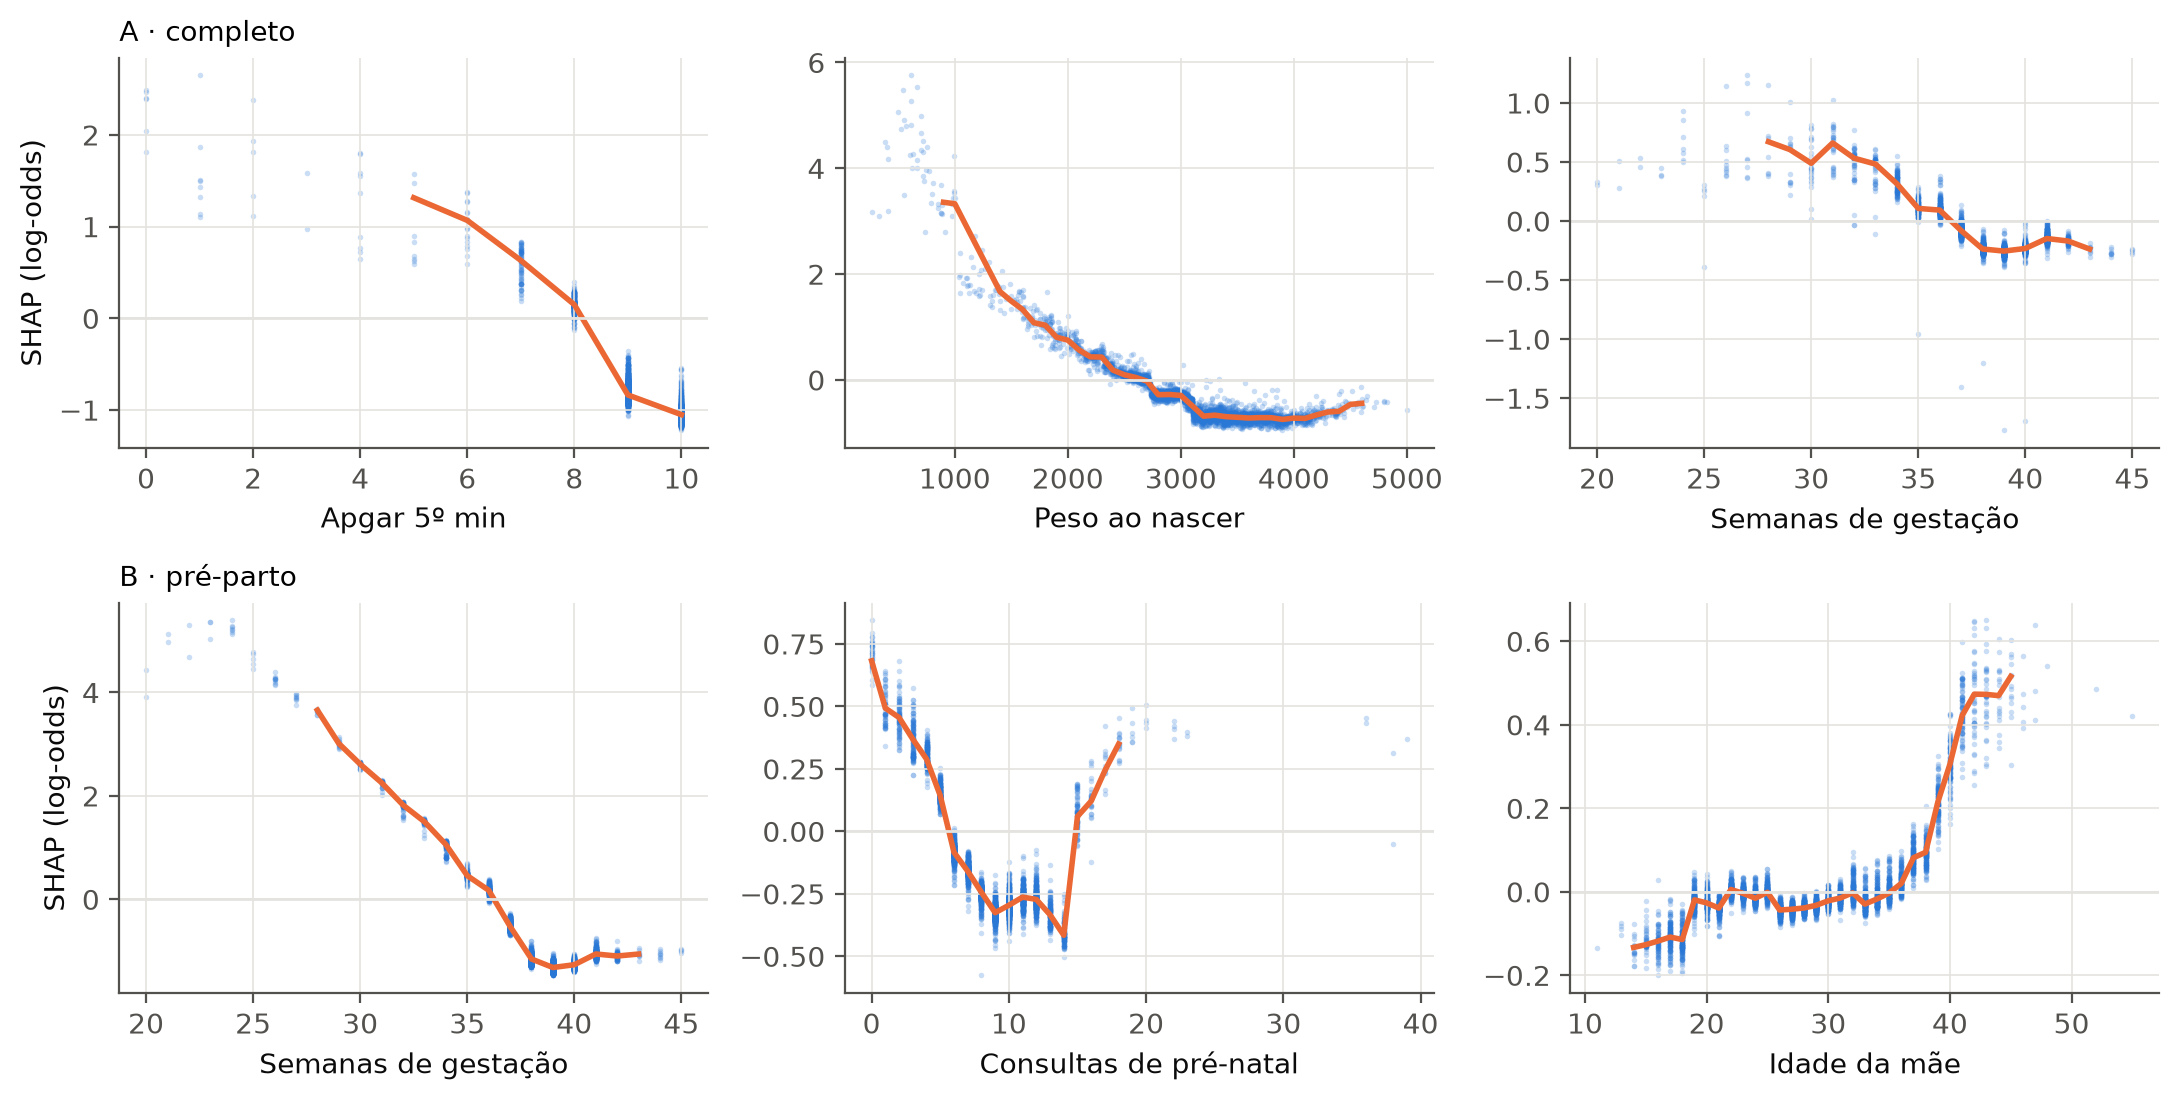
\includegraphics[width=0.85\textwidth]{xai_dependencia.png}
\caption{Dependência SHAP: contribuição (log-odds) em função do valor da variável; a linha é a mediana por valor.}
\label{fig:dep}
\end{figure}

\begin{figure}[!htbp]
\centering
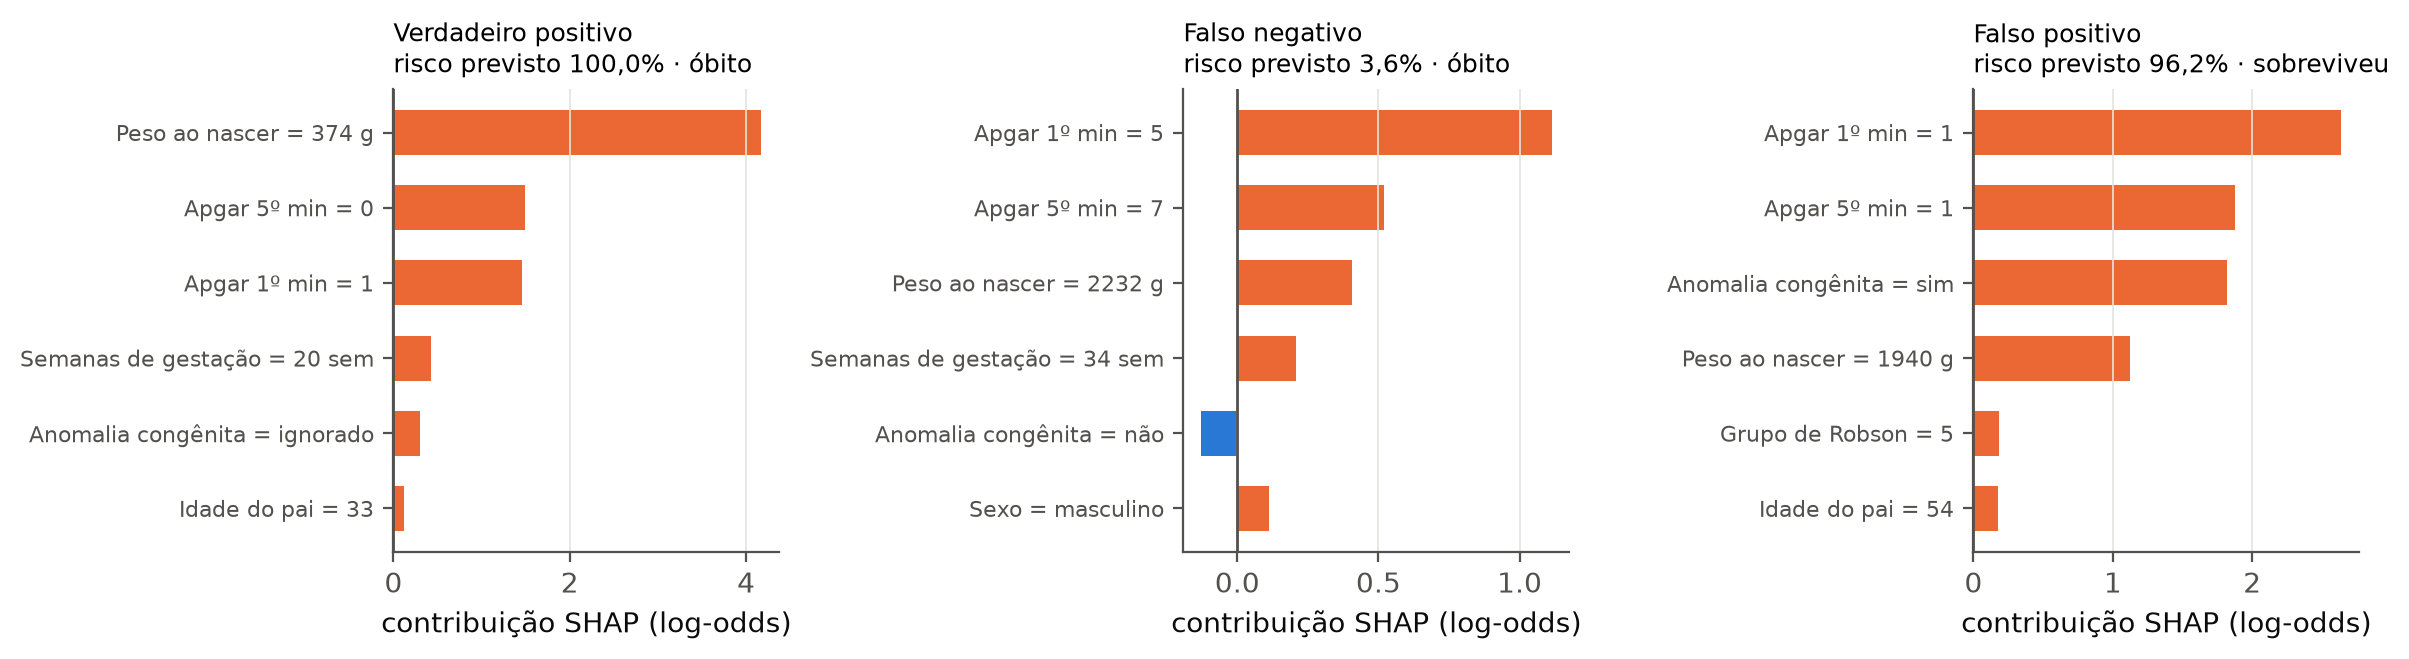
\includegraphics[width=\textwidth]{xai_local.png}
\caption{Explicações locais (SHAP) de três casos do teste de \anoTeste{}, no modelo A: as 6 maiores contribuições.}
\label{fig:local}
\end{figure}

\subsection{Calibração, utilidade clínica e subgrupos}

\textbf{Calibração.} A curva de calibração (Figura~\ref{fig:dca}, à esquerda) acompanha a diagonal nas faixas de maior risco, e as inclinações são próximas de 1 (recalibrados: intercepto \calACalInt{} e inclinação \calACalInc{} no A; \calBCalInt{} e \calBCalInc{} no B).
A recalibração foi \emph{indispensável}. A busca escolheu o peso de classe $\sqrt{n_0/n_1} \approx$ \spwA{} para o XGBoost, e com isso o escore bruto superestima muito o risco: O/E de \oeBrutoA{} (A) e \oeBrutoB{} (B), intercepto de \calABruInt{} (curvas pontilhadas). A isotônica corrige isso para \AXgbOE{} e \BXgbOE{}. A leve superestimação que resta (interceptos negativos) é compatível com o \emph{drift}: a isotônica foi ajustada em \anoValid{}, quando a TMN foi de \tmnValid{}‰, e no teste ela caiu para \tmnTeste{}‰. É uma explicação plausível, não uma prova, porque a magnitude não coincide exatamente.

\textbf{Utilidade clínica.} Com prevalência de 0,8\%, a estratégia de tratar todos tem benefício negativo em qualquer limiar acima de 0,8\%, então a comparação relevante é com não intervir. A faixa de limiares foi escolhida pelo uso clínico: para uma transferência \emph{in utero} ou a priorização de UTI neonatal, é plausível aceitar de 9 a 49 falsos alarmes por óbito identificado, o que corresponde a $p_t$ entre 2\% e 10\%. Nessa faixa (Figura~\ref{fig:dca}, à direita), o benefício líquido do modelo A vai de \nbADois{} a \nbADez{} por mil nascidos vivos, e o do B, de \nbBDois{} a \nbBDez{}, sempre acima de zero. O máximo possível é a própria TMN, \tmnTeste{}.

\textbf{H3.} A hipótese previa pior calibração na baixa escolaridade. Mas o O/E de mães com fundamental incompleto foi de \subBFundOE{} no modelo B e \subAFundOE{} no A, com IC que incluem 1 e se sobrepõem aos do ensino superior (\subBSupOE{} em B), então H3 não se confirmou. Os subgrupos (figura no material suplementar) mostram dois achados:
\begin{itemize}
  \item \textbf{Discriminação:} no modelo A, ela é pior na baixa escolaridade, com AUROC de \subAFundAuroc{} contra \subASupAuroc{} no ensino superior e IC que não se sobrepõem.
  \item \textbf{Calibração:} no modelo A, os O/E ficam abaixo de 1 na maioria dos subgrupos, refletindo a leve superestimação global (O/E \AXgbOE{}). Ela é mais marcada na capital (\subACapOE{}) e no ensino superior (\subASupOE{}); nenhum subgrupo é subestimado. No teste de \anoTesteAnt{}, os achados eram outros: o modelo B subestimava mães brancas (O/E \antBBrancaOE{}) e o interior (\antBIntOE{}), e no teste de \anoTeste{} isso não se repetiu (\subBBrancaOE{} e \subBIntOE{}). Diferenças de calibração por subgrupo são, portanto, instáveis de um ano para outro.
\end{itemize}

\begin{figure}[!htbp]
\centering
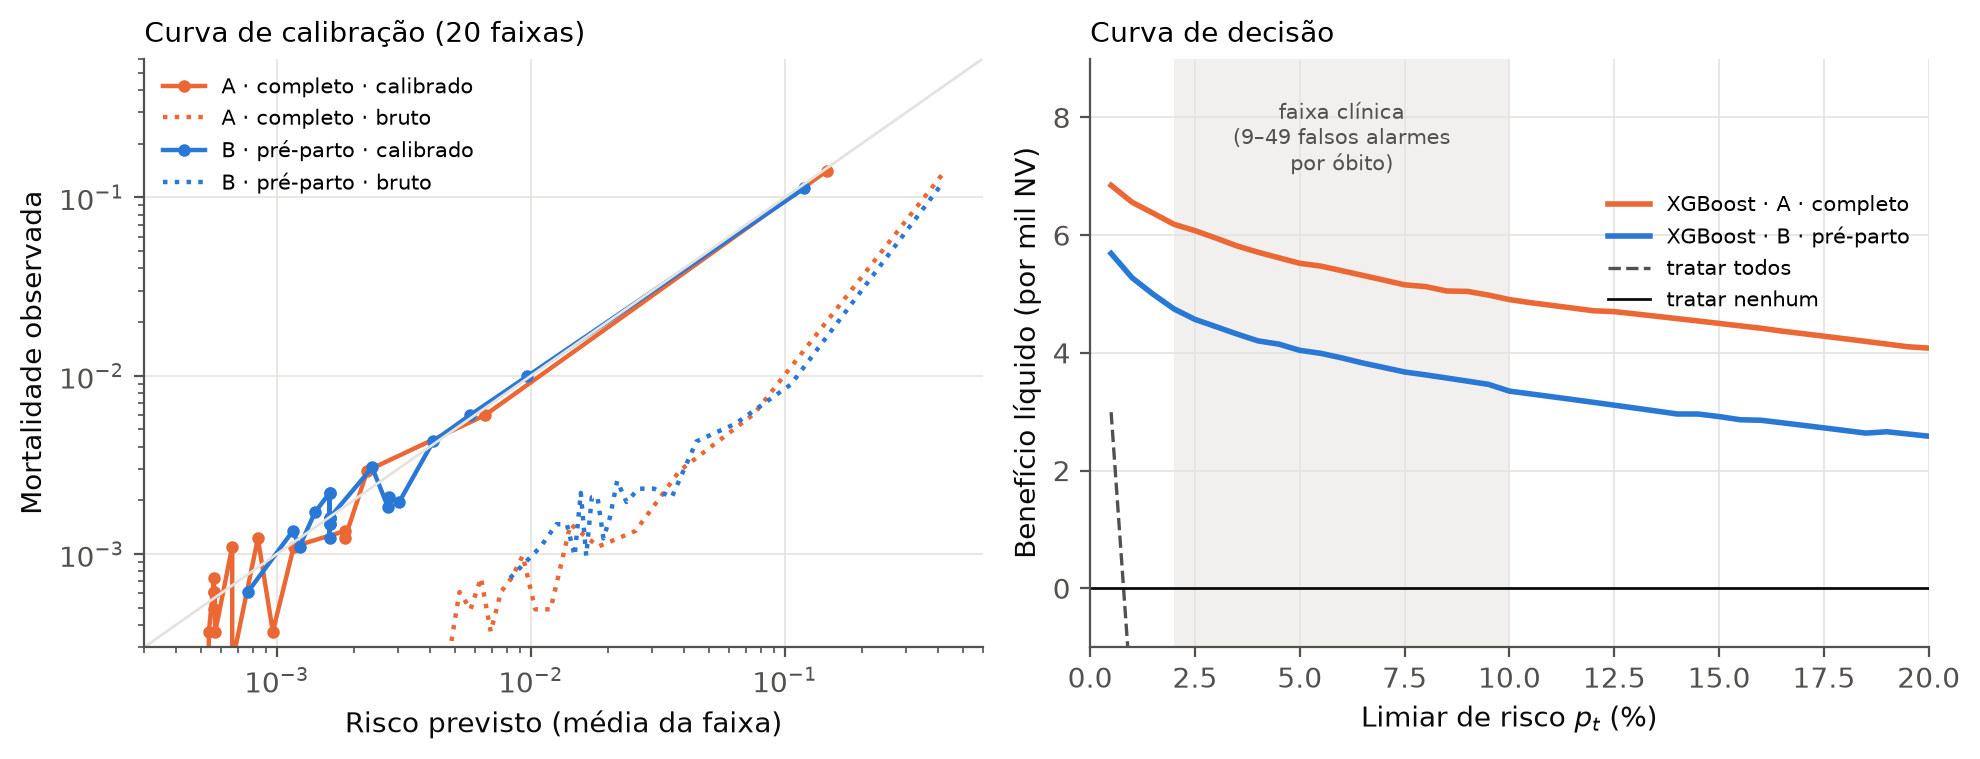
\includegraphics[width=0.95\textwidth]{calibracao_decisao.png}
\caption{Teste de \anoTeste{}. Esquerda: curva de calibração em 20 faixas de risco (escala log), com probabilidade recalibrada (linha cheia) e bruta (pontilhada). Direita: curva de decisão, com benefício líquido por mil nascidos vivos e faixa clínica sombreada.}
\label{fig:dca}
\end{figure}

\subsection{Sensibilidade ao linkage}
\label{sec:v1fim}

O XGBoost foi reajustado com os mesmos hiperparâmetros e rótulos alternativos no ajuste e na validação: \textbf{estrito}, sem os nascimentos pareados nas passadas 3--6, e \textbf{pior caso}, com esses nascimentos rotulados como sobreviventes. Os dois foram avaliados no \emph{mesmo} teste de \anoTeste{} completo, com $\Delta$ por bootstrap pareado. A discriminação praticamente não muda: $\Delta$AUROC = \sensAEstDelta{} (estrito) e \sensAPiorDelta{} (pior caso) no modelo A, e \sensBEstDelta{} e \sensBPiorDelta{} no B. Isso mostra que o modelo é robusto a ruído de rótulo \emph{no treino}. Já o O/E sobe para \sensAEstOE{}--\sensBPiorOE{}, porque com menos positivos no treino o modelo aprende uma prevalência menor.

O \emph{teste} também tem rótulos imperfeitos. Avaliando o modelo principal sem os pares tolerantes do teste, a AUROC é de \testeEstrAAuroc{} (A) e \testeEstrBAuroc{} (B); marcando-os como sobreviventes, é de \testeZeroAAuroc{} e \testeZeroBAuroc{}. Os pares tolerantes não inflam a AUROC reportada. Já os $\approx$10\% de óbitos sem nenhum par não podem ser avaliados, o que é um limite da validação.

% ---------------------------------------------------------------------------
\section{Aprofundamento (v2): questões para publicação}
\label{sec:v2}

Todas as análises desta seção reaproveitam os hiperparâmetros do experimento principal e, salvo indicação, avaliam no \emph{mesmo} teste de \anoTeste{}, com $\Delta$ por bootstrap pareado. O código está em \texttt{src/aprofundamento.py}.

\subsection{Q1: um escore clínico simples basta?}

Ajustamos regressões logísticas só com peso, idade gestacional e Apgar 5, e com essas três mais a anomalia congênita, escolhendo $C$ e recalibrando em \anoValid{} como no modelo principal (Tabela~\ref{tab:v2base}).

\begin{table}[!htbp]
\centering
\caption{Q1: escores simples $\times$ XGBoost completo (teste de \anoTeste; $\Delta$ por bootstrap pareado).}
\label{tab:v2base}
\small
\setlength{\tabcolsep}{4pt}
\tabVBaseline
\end{table}

Com três variáveis, a AUROC foi de \vBaseTresAuroc{}, a \vBaseTresDauroc{} do XGBoost. Com a anomalia, subiu para \vBaseQuatroAuroc{}, a só \vBaseQuatroDauroc{}, e os 5\% de maior risco concentraram \vBaseQuatroTop{} dos óbitos. A diferença que resta está na AUPRC: \vBaseQuatroAuprc{} contra \AXgbAuprc{} ($\Delta$ = \vBaseQuatroDauprc{}). \textbf{Resposta:} quase toda a ordenação vem de quatro campos da DN; o ganho do XGBoost se concentra na precisão entre os nascimentos de maior risco. A contribuição do trabalho, portanto, não é o algoritmo, e sim os dados abertos, o linkage, a calibração e a avaliação de equidade.

\subsection{Q2: há vazamento na DN?}

A DN deveria ser preenchida no nascimento. Se campos como a anomalia fossem completados depois do óbito, as DN preenchidas depois seriam previstas melhor. Testamos isso de duas formas.

\textbf{Por idade no óbito.} Cada faixa foi comparada com todos os sobreviventes do teste. A AUROC do modelo A cai de \vIdadeAZero{} no dia 0 para \vIdadeAUm{} entre 1 e 6 dias e \vIdadeASete{} entre 7 e 27 dias (Figura~\ref{fig:v2idade}). O mesmo gradiente aparece no modelo B (\vIdadeBZero{}, \vIdadeBUm{} e \vIdadeBSete{}), que não tem Apgar nem anomalia. Ele reflete, portanto, a gravidade: quem morre no dia 0 é, em geral, extremamente prematuro.

\begin{figure}[!htbp]
\centering
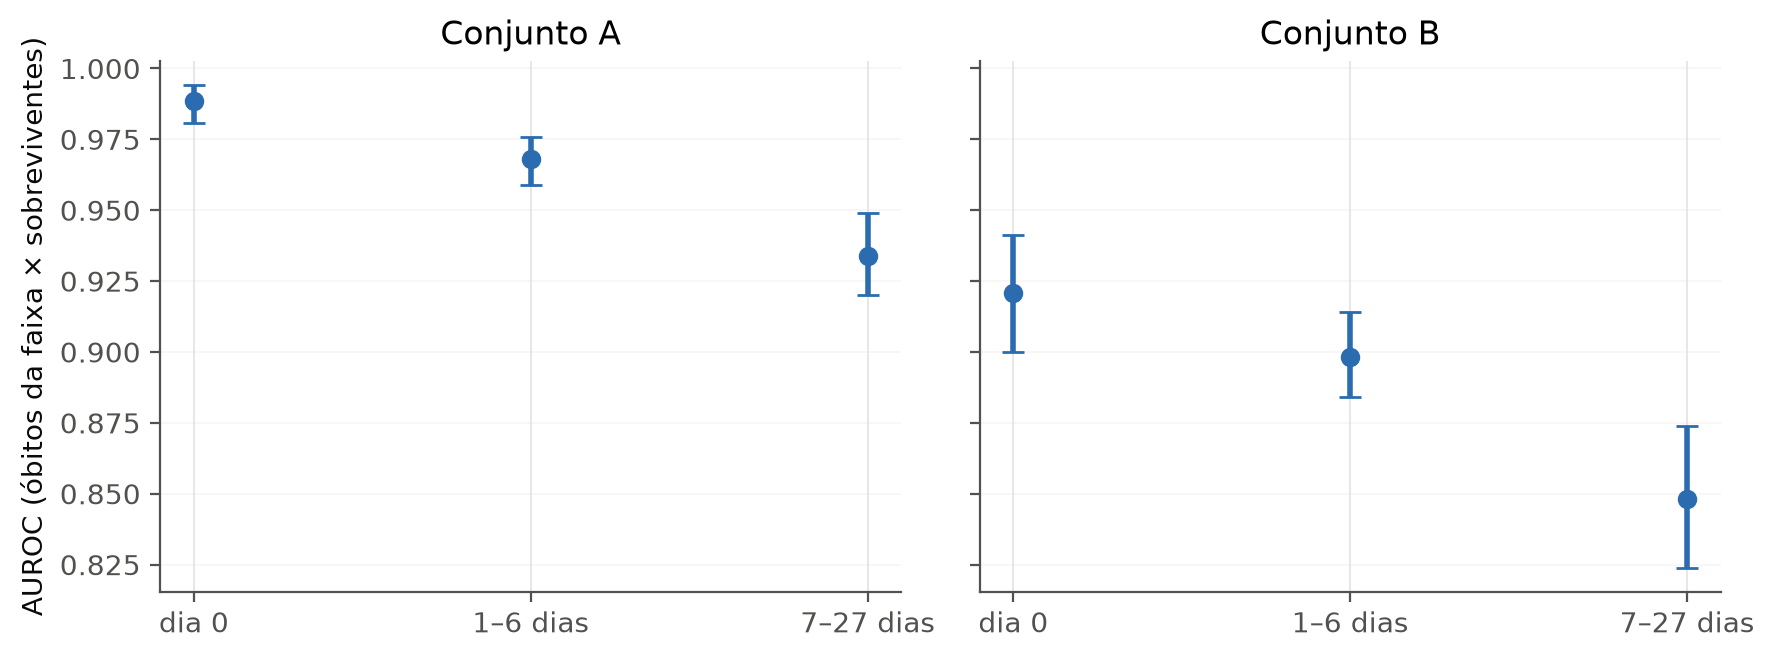
\includegraphics[width=0.8\textwidth]{v2_idade_obito.png}
\caption{Q2: AUROC por faixa de idade no óbito (óbitos da faixa $\times$ todos os sobreviventes), com IC 95\%.}
\label{fig:v2idade}
\end{figure}

\textbf{Pela data da declaração.} A DN traz a data em que foi preenchida (\texttt{DTDECLARAC}). No teste, \vDecPct{} dos óbitos (\vDecN) tiveram a DN declarada depois do óbito, e \vDecPctZero{} no dia 0. A digitação (\texttt{DTCADASTRO}) é posterior ao óbito em \vDigPct{} dos casos e por isso não discrimina. Comparamos os dois grupos dentro da mesma faixa de idade, o que controla a gravidade (Tabela~\ref{tab:v2dec}). No dia 0, a AUROC foi de \vDecAZeroDep{} com DN declarada depois e \vDecAZeroAnt{} com DN declarada até o dia do óbito, com IC sobrepostos. Entre 1 e 6 dias, a diferença foi maior (\vDecAUmDep{} contra \vDecAUmAnt{}, com só \vDecAUmDepN{} óbitos no primeiro grupo), mas apareceu igualmente no modelo B (\vDecBUmDep{} contra \vDecBUmAnt{}), que não contém os campos que poderiam ser preenchidos com conhecimento do óbito. \textbf{Resposta:} não há evidência de vazamento além da gravidade.

\begin{table}[!htbp]
\centering
\caption{Q2: AUROC dos óbitos com DN declarada depois do óbito $\times$ até o dia do óbito, na mesma faixa de idade (contra todos os sobreviventes).}
\label{tab:v2dec}
\small
\tabVDeclaracao
\end{table}

\subsection{Q3 e Q4: pandemia e variáveis de chave}

Reajustamos o XGBoost sem 2020--2021 no ajuste (Q3) e sem as cinco variáveis que também entram nas chaves do linkage: peso, idade da mãe, semanas, gravidez e parto (Q4). A Tabela~\ref{tab:v2rob} mostra os resultados.

\begin{table}[!htbp]
\centering
\caption{Q3 e Q4: XGBoost reajustado com os mesmos hiperparâmetros (teste de \anoTeste; $\Delta$ por bootstrap pareado).}
\label{tab:v2rob}
\small
\setlength{\tabcolsep}{4pt}
\tabVRobustez
\end{table}

\textbf{Q3.} Sem os anos de pandemia, $\Delta$AUROC = \vPandADauroc{} (A) e \vPandBDauroc{} (B), com IC que incluem zero. A pandemia não distorceu o treino.

\textbf{Q4.} No modelo A, sem as variáveis de chave, a AUROC cai pouco ($\Delta$ = \vChaveADauroc{}), porque o Apgar e a anomalia carregam boa parte da informação, mas a AUPRC cai muito ($\Delta$ = \vChaveADauprc{}). No modelo B, a queda é grande: AUROC de \vChaveBAuroc{} ($\Delta$ = \vChaveBDauroc{}), porque sai a idade gestacional. O modelo pré-parto depende, portanto, de um campo que também define quem recebe rótulo. Como a sensibilidade da Seção~\ref{sec:v1fim} mostrou que os pares tolerantes não alteram a discriminação, essa dependência não parece criar um artefato; mas ela reforça que erros na idade gestacional afetam ao mesmo tempo o linkage e a predição.

\subsection{Q5: janelas temporais e \emph{drift}}

Para cada ano de teste $t$ entre \vJanAnoIni{} e \vJanAnoFim{}, o modelo foi ajustado até $t-2$, recalibrado em $t-1$ e testado em $t$ (\emph{reajustado}). O modelo \emph{congelado} é o da primeira janela (ajuste em 2017--2018), aplicado aos anos seguintes sem reajuste nem recalibração (Figura~\ref{fig:v2jan}).

\begin{figure}[!htbp]
\centering
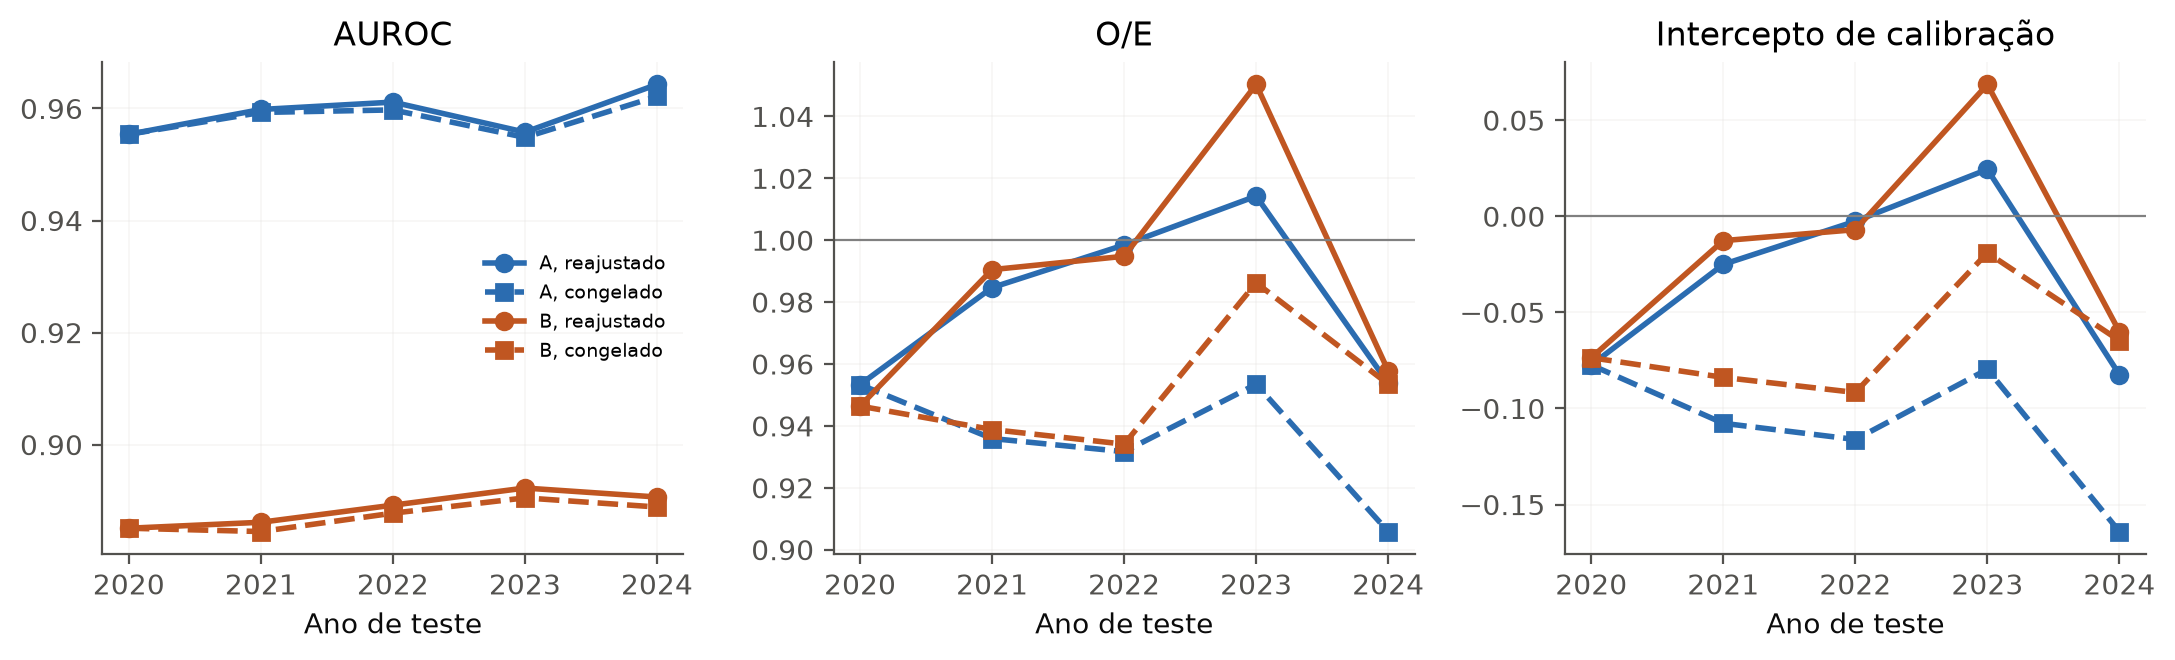
\includegraphics[width=\textwidth]{v2_janelas.png}
\caption{Q5: AUROC, O/E e intercepto de calibração por ano de teste; modelo reajustado todo ano (linha cheia) $\times$ congelado desde a primeira janela (tracejada).}
\label{fig:v2jan}
\end{figure}

A discriminação é estável: a AUROC do modelo A reajustado ficou entre \vJanAAurocMin{} e \vJanAAurocMax{}, e a do congelado, em \vJanACongAurocUlt{} no último ano. A calibração, não. O O/E do modelo reajustado oscilou entre \vJanAOeMin{} e \vJanAOeMax{}, acompanhando a TMN de cada ano, e o do congelado caiu até \vJanACongOeUlt{} em \vJanAnoFim{} (intercepto \vJanACongIntUlt{}), superestimando o risco de forma crescente. \textbf{Resposta:} o modelo não precisa ser retreinado para ordenar bem, mas precisa ser recalibrado periodicamente. Uma ressalva: o modelo congelado também foi ajustado com menos anos.

\subsection{Q6: simulação de padrão-ouro do linkage}

Sem acesso à base identificada, fabricamos uma verdade conhecida. As DN dos \nPareados{} nascidos efetivamente pareados viraram ``DO sintéticas'', com a taxa de ausência de cada campo observada nas DO reais e erros por campo em três cenários (baixo, realista e alto: peso $\pm$10--100~g, idade da mãe $\pm$1 ano, semanas $\pm$1--2, estabelecimento trocado por transferência). O linkage rodou contra toda a base, e os demais nascidos serviram de distratores. Em dois cenários adicionais, 5\% e 10\% das DN verdadeiras foram retiradas da base, simulando sub-registro ou residência diferente na DN e na DO (Tabela~\ref{tab:v2sim} e Figura~\ref{fig:v2sim}).

\begin{table}[!htbp]
\centering
\caption{Q6: falsos pares reais e estimados pelo modelo de mistura, por passada e cenário, e desempenho da etapa probabilística (FS).}
\label{tab:v2sim}
\small
\setlength{\tabcolsep}{4pt}
\tabVSimulacao
\end{table}

\begin{figure}[!htbp]
\centering
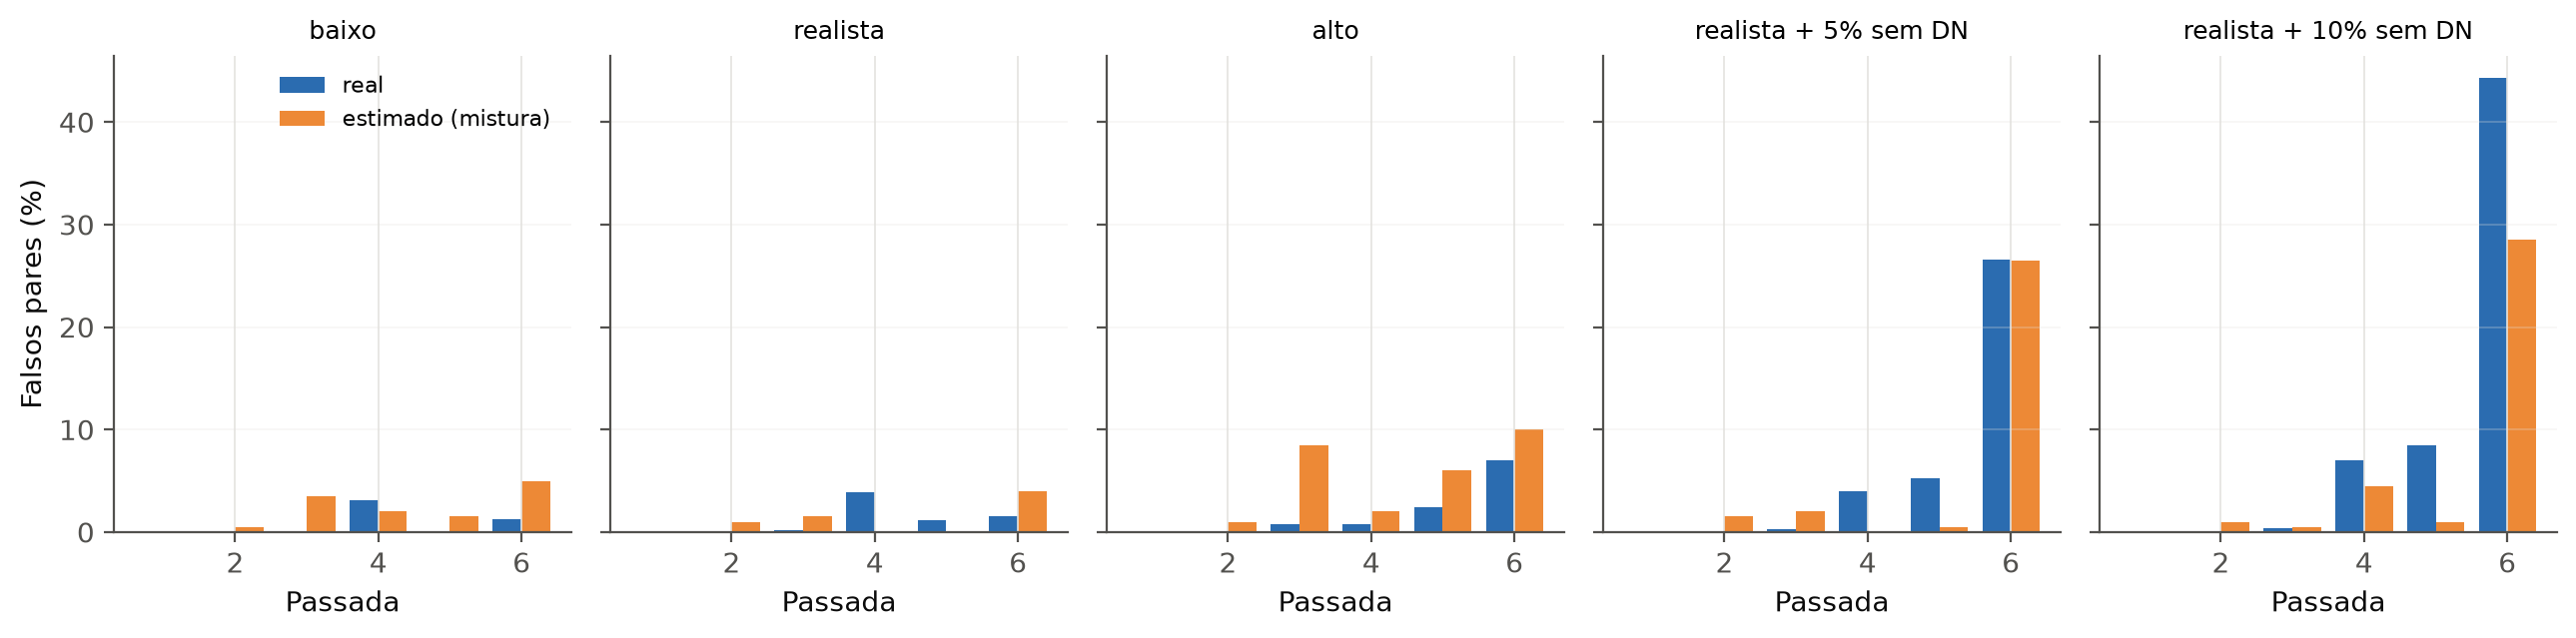
\includegraphics[width=\textwidth]{v2_simulacao.png}
\caption{Q6: fração real (azul) e estimada (laranja) de falsos pares por passada, em cada cenário da simulação.}
\label{fig:v2sim}
\end{figure}

Três resultados:
\begin{itemize}
  \item \textbf{Quando a DN verdadeira existe, a cascata é precisa.} Mesmo no cenário de ruído alto, os falsos pares ficaram em \vSimAltoFalsos{} no total e no máximo \vSimAltoMaxTol{} numa passada, e \vSimAltoCob{} dos óbitos receberam o par verdadeiro.
  \item \textbf{A DN ausente concentra os falsos pares na chave mais tolerante.} Com 5\% e 10\% das DN ausentes, a passada 6 chegou a \vSimSemCincoSeis{} e \vSimSemDezSeis{} de falsos pares, porque o óbito sem DN acaba pareado com um nascido parecido do mesmo hospital.
  \item \textbf{O estimador de mistura é impreciso.} Ele acompanha a ordem de grandeza, mas erra por vários pontos nas passadas pequenas e \emph{subestima} os falsos pares quando há DN ausente (passada 6 com 10\% ausentes: \vSimSemDezSeis{} reais contra \vSimSemDezSeisEst{} estimados). Nos dados reais, porém, ele estima 17--31\% na passada 3, valor que nenhum cenário reproduz. Uma explicação é que a premissa de concordância constante ($c_{\text{verd}}$ igual em todas as passadas) falha quando os registros das passadas tolerantes também têm escolaridade e perdas fetais mais mal preenchidas, o que infla a estimativa. As taxas estimadas na primeira parte devem ser lidas como ordem de grandeza, não como medida.
\end{itemize}

\subsection{Q7: etapa probabilística (Fellegi--Sunter)}

Sobre os \vFsRestantes{} óbitos que a cascata não pareou, comparamos cada óbito com os nascidos ainda livres da mesma data e sexo (\vFsCand{} pares candidatos). Cada campo recebe um nível de concordância: exato; próximo (peso $\pm$50~g, idade da mãe e semanas $\pm$1); discorda; ou ausente, que não pesa. O peso do par é
\begin{equation}
w = \sum_j \log_2 \frac{m_j(\gamma_j)}{u_j(\gamma_j)}, \qquad
P(\text{par}\mid\gamma) = \frac{1}{1 + 2^{-(w + \log_2[\lambda/(1-\lambda)])}},
\end{equation}
com $u_j$ estimado em pares aleatórios do mesmo bloco e $m_j$ nos pares determinísticos em cujas chaves o campo não entra. A proporção $\lambda$ = \vFsLambda{} supõe no máximo um par verdadeiro por óbito no bloco. Pares com probabilidade $\geq$ 0,9 foram aceitos 1:1, do mais provável para o menos provável~\cite{fellegi1969}. O EM, alternativa usual para $m$ e $\lambda$, convergiu para $\lambda$ = \vFsEmLambda{}, dez vezes o plausível: separou ``mesmo município'' de ``outro município'', e não pares de não pares.

A etapa aceitou só \vFsN{} pares, com falsos pares estimados de \vFsFalsos{}, e nenhum no teste. Os óbitos restantes não são recuperáveis: \vFsPostBaixoPct{} deles não têm nenhum candidato com probabilidade acima de 0,1, e \vFsCompletos{} têm os sete campos preenchidos na DO e ainda assim não encontram par. Isso aponta para DN ausente da base, e não para campos faltantes. Na simulação, o mesmo padrão aparece: a etapa FS gera poucos pares, e com 5--10\% de DN ausentes a maioria é falsa (\vSimSemCincoFsFalsos{} e \vSimSemDezFsFalsos{}). \textbf{Resposta:} com os campos da DO pública, uma etapa probabilística não recupera o resíduo, e o limite do linkage não é o método, e sim a existência da DN na base do mesmo estado.

% ---------------------------------------------------------------------------
\section{Discussão}

\textbf{H1 foi confirmada.} Com dados abertos, o XGBoost teve AUROC de \AXgbAuroc{} e concentrou \AXgbTop{} dos óbitos nos 5\% de maior risco, contra 0,971 e mais de 90\% no artigo, com as mesmas cinco variáveis principais. O modelo é robusto a ruído de rótulo no treino, e os pares duvidosos do teste não inflam a AUROC. Não é possível descartar, porém, um viés vindo dos óbitos que ficaram sem par.

A diferença residual para o artigo é compatível com três fatores: os $\approx$15\% de óbitos sem par verdadeiro, de perfil diferente (mais ausências, mais do interior, mais óbitos precoces fora do hospital); a heterogeneidade do estado; e a pior qualidade da DN e da DO no interior.

\textbf{H2 foi confirmada em parte.} Houve queda real ($\Delta$AUROC = \dAB{}, $\Delta$AUPRC = \dABprc{}), mas o modelo B manteve AUROC de \BXgbAuroc{} e benefício líquido positivo, quase tudo pela idade gestacional. O uso adequado é delimitado: estimar, na admissão para o parto, o risco dado que o nascimento ocorre agora. Isso apoia a decisão sobre transferência \emph{in utero} para uma maternidade com UTI neonatal e o preparo da equipe. O modelo não serve para triagem precoce da gestação, porque a idade gestacional do parto e as consultas acumuladas não são conhecidas semanas antes.

\textbf{H3 não foi confirmada.} A calibração na baixa escolaridade não foi pior. O achado de equidade que se sustenta é outro: no modelo A, a \emph{discriminação} é menor para filhos de mães com fundamental incompleto. Uma hipótese é que a DN desses nascimentos tenha pior qualidade de preenchimento. Já as diferenças de calibração por subgrupo mudaram entre os testes de \anoTesteAnt{} e \anoTeste{}, o que desaconselha interpretá-las como viés estrutural.

Para capital e interior, testamos o linkage diferencial. O pareamento é menor no interior (\linkInt{} contra \linkCap{}), mas quase não mudou entre os anos, e por si só deslocaria o O/E em menos de 2\% (Tabela~\ref{tab:comp}). Ele não explica a diferença observada (\oeRegACapCal{} contra \oeRegAIntCal{} no modelo A).

Para raça/cor, o pareamento é quase uniforme, mas a evidência é indireta, porque usa a raça do recém-nascido, e não a da mãe. \cite{ramos2025} encontraram captura equivalente entre grupos, o que é coerente com a nossa discriminação próxima entre grupos de raça/cor (AUROC de \subABrancaAuroc{} para mães brancas e \subAPretaAuroc{} para pretas, no modelo A).

\textbf{Calibração e \emph{drift}.} Com o peso de classe escolhido pela busca, a calibração depende inteiramente da etapa isotônica. Depois dela, a curva e a inclinação $\approx$ 1 indicam boa calibração. A calibração absoluta, porém, depende de fatores externos ao modelo: a completude do linkage, vista na sensibilidade, e a variação anual da TMN (\tmnValid{}‰ em \anoValid{} e \tmnTeste{}‰ em \anoTeste{}). Em uso real, seria preciso recalibrar o intercepto periodicamente.

\textbf{O que a v2 muda na leitura.} As perguntas da Seção~\ref{sec:v2} deslocam a contribuição do trabalho. (i) O algoritmo importa pouco para a ordenação: quatro campos da DN chegam a \vBaseQuatroAuroc{} de AUROC, e o ganho do XGBoost está na AUPRC. (ii) O desempenho não é artefato de vazamento, da pandemia nem dos pares tolerantes. (iii) O modelo ordena de forma estável ao longo dos anos, mas a calibração deriva, o que torna a recalibração anual parte do modelo, e não um detalhe. (iv) O linkage sem identificadores é preciso quando a DN existe na base, e o resíduo de $\approx$10\% não se recupera com métodos probabilísticos. A causa provável é a DN ausente do arquivo do mesmo estado, por sub-registro ou por residência declarada de forma diferente na DN e na DO. Isso muda o próximo passo: em vez de sofisticar o pareamento, é preciso ampliar a base de busca, por exemplo pareando o resíduo com as DN das UF vizinhas.

\textbf{Limitações.} Os rótulos são imperfeitos ($\approx$15\% dos óbitos sem par verdadeiro); a validação é temporal, mas não externa; o modelo A usa variáveis posteriores ao nascimento; o bootstrap ignora a dependência entre gêmeos; a calibração por subgrupo varia de um ano para outro; o SIM \anoObFim{} ainda é preliminar; não houve óbitos suficientes para analisar mães amarelas e indígenas; e a simulação de padrão-ouro depende de premissas sobre o tipo e a taxa de erro dos campos, que só uma base identificada pode confirmar.

% ---------------------------------------------------------------------------
\section{Conclusão}

É possível reproduzir, só com dados abertos, um modelo brasileiro de predição de mortalidade neonatal com discriminação próxima à publicada, e essa discriminação é robusta a ruído de rótulo no treino. As explicações SHAP são aditivas, estáveis e clinicamente plausíveis. A calibração absoluta, ao contrário, é sensível ao linkage e ao \emph{drift} temporal. Um modelo na admissão para o parto mantém AUROC de \BXgbAuroc{} e benefício líquido positivo, para decisões de transferência \emph{in utero}.

Na versão 2, o trabalho resistiu às perguntas de um revisor: não há sinal de vazamento, a pandemia não distorce o treino, a discriminação é estável no tempo e a cascata determinística é precisa quando a DN existe. Por outro lado, a v2 mostrou que um escore com quatro campos da DN chega perto do XGBoost, que a calibração exige atualização anual e que o resíduo do linkage não se recupera com uma etapa probabilística.

Como trabalhos futuros, ficam:
\begin{itemize}
  \item parear o resíduo de óbitos com as DN das UF vizinhas, para testar a hipótese de DN fora da base;
  \item validar o linkage e o estimador de falsos pares contra uma base identificada (SES-RJ ou CIDACS/Fiocruz);
  \item fazer a validação externa em outras UFs, com treino numa região e teste em outra;
  \item usar o tipo de anomalia congênita (\texttt{CODANOMAL});
  \item avaliar o impacto junto à rede de atenção materno-infantil.
\end{itemize}

\textbf{Reprodutibilidade.} O código, os testes, o notebook, os geradores deste relatório e dos slides e o manifesto dos dados estão em \url{\repo}. O comando \texttt{python -m src.experimento} refaz todos os números da primeira parte a partir do FTP do DATASUS, e \texttt{python -m src.aprofundamento}, os da Seção~\ref{sec:v2}. A versão 1 está marcada no repositório com a tag \texttt{v1.0}.

\bibliographystyle{sbc}
\bibliography{refs}

\end{document}
